% ===========================================================================
%  IntroAct-TS —— ICLR 2027 投稿正文
% ---------------------------------------------------------------------------
%  版本      : v4.6（2026-09-19）
%  上一版    : IntroActTS_20260918_v45_review.tex（占位符骨架，已冻结存档）
%
%  本版与 v4.5 的差别
%  -----------------
%  1. 数字来自 v4.6 的独立 TEST 运行：8 个来源、95 个 TEST parent、760 个
%     episode、三个冻结骨干、四种缺失模式、三档严重度。结果记录在
%     results/v46/，表格与解读文字由 latex/fill_v46.py 从那些 JSON 生成，
%     所以数字和围绕它的句子不会各自漂移。
%  2. 仍未跑出的量保留 \ph{KEY} 占位符，渲染为灰色 [KEY]，绝不用估计值填充。
%  3. 主表 roster：Native KEEP / Best Fixed / R2-CART / SAITS / TATO 加
%     IntroAct-TS，Catalog Oracle 只作诊断。没有可运行公开实现、或其方法
%     前提与冻结骨干不相容的方法一律不进任何表，逐条记录在附录 B.1。
%  4. 选参改为在 replay bank 上做留一 parent 交叉验证，约束是条件有害率不
%     超过最佳固定干预的条件有害率；(k, beta) 逐骨干选。
%  5. 结论措辞与实测一致：只在成立的骨干上声称成立，不成立处如实写出。
%
%  维护方式：改这个文件，然后跑 python latex/fill_v46.py 生成
%  latex/IntroActTS_20260919_v46_filled.tex 和 PDF。
% ===========================================================================
\documentclass{article}

\usepackage{iclr2027_conference,times}
\input{math_commands.tex}

\usepackage{hyperref}
\usepackage{url}
\usepackage{graphicx}
\usepackage{booktabs}
\usepackage{amsmath}
\usepackage{amssymb}
\usepackage{multirow}
\usepackage{array}
\usepackage[table]{xcolor}

% ---------------------------------------------------------------- 版式与宏
\definecolor{phgray}{gray}{0.45}
\definecolor{bestgray}{gray}{0.94}

% 未运行结果的占位符。KEY 一律用下划线分层命名（如 MAIN_OVERALL_MASE），
% 下划线是数学下标字符，因此必须 \detokenize 成普通字符后才能进 \textsf。
% 填充时只替换 KEY，不要改 \ph 本身。
\newcommand{\ph}[1]{\textcolor{phgray}{\textsf{[\detokenize{#1}]}}}
% 表格中强调：第一名加粗，第二名下划线，Oracle 用斜体灰字。
\newcommand{\best}[1]{\textbf{#1}}
\newcommand{\second}[1]{\underline{#1}}
\newcommand{\oracle}[1]{\textit{\textcolor{phgray}{#1}}}
\newcommand{\introact}{\textsc{IntroAct-TS}}
\newcommand{\tsfm}{TSFM}
\newcommand{\calA}{\mathcal{A}}
\newcommand{\calB}{\mathcal{B}}
\newcommand{\calN}{\mathcal{N}}
\newcommand{\loss}{\ell}

\newcommand{\fix}{\marginpar{FIX}}
\newcommand{\new}{\marginpar{NEW}}

% ICLR 正文硬上限 9 页，浮动体间距默认偏松，这里收紧以腾出正文空间。
\setlength{\textfloatsep}{7pt plus 2pt minus 2pt}
\setlength{\floatsep}{7pt plus 2pt minus 2pt}
\setlength{\intextsep}{7pt plus 2pt minus 2pt}
% 正文有 6 张表 + 5 张图，默认每页浮动体上限会让它们堆积到最后一页。
% 放宽每页浮动体配额，让它们均匀分布在第 1-9 页内。
\setcounter{topnumber}{4}
\setcounter{bottomnumber}{3}
\setcounter{totalnumber}{5}
\renewcommand{\topfraction}{0.92}
\renewcommand{\bottomfraction}{0.65}
\renewcommand{\textfraction}{0.06}
\renewcommand{\floatpagefraction}{0.72}

\title{\introact{}: Selective Input Governance for \\
Frozen Time-Series Foundation Models}

\author{Anonymous Authors\\Paper under double-blind review}

%\iclrfinalcopy
\begin{document}

\maketitle

\begin{abstract}
A time-series foundation model is deployed without task-specific parameter updates, so when the
context it receives at forecast time is incomplete, the only thing a deployment can still
change is the input. Existing methods reconstruct the unavailable values or train an
architecture that tolerates missingness, and both options are closed once the forecaster is
frozen. The question we study is which of several admissible ways of handling an incomplete
context should be applied to the current request, and whether any should be applied at all. We
introduce \introact{}. It replays historical windows as pseudo-deployments, executes every
admissible action with the frozen forecaster to measure what that action actually did to the
forecast, and stores the result. A new request is scored against the stored evidence of the
same action, and an action runs only when a conservative utility estimate is positive.
Keeping the input unchanged is one of the actions, so the method returns the original forecast
whenever the evidence does not support a change, and every forecast it returns comes from an
input version that was actually executed. Across eight sources, four missingness
patterns and two horizons, on two frozen backbones used for development and a third family
held out from method design, \introact{} lowers source-macro MASE from 1.576 to 1.447, improves on the untouched input on every backbone with paired intervals that exclude zero, and has the best average rank of the deployable rows on every backbone. The evidence says that for a frozen forecaster the useful question about an incomplete input is which repair to run on this request, and that the answer can be read off what past repairs did to this forecaster.
\end{abstract}

% ===========================================================================
\section{Introduction}
\label{sec:intro}

Time-series foundation models (\tsfm{}s) now produce competitive zero-shot forecasts without
task-specific retraining~\citep{ansari2024chronos,chronosbolt2025,das2024timesfm,woo2024moirai,
chronos2_2025}, which makes them attractive as fixed components of deployed forecasting
systems. The context available at the forecast origin is often
incomplete~\citep{chen2024bitgraph,peng2025s4m}. A sensor stops reporting for a stretch of
time, a channel delivers a variable several steps late, or only part of an acquisition batch
has arrived. We study deployment protocols in which an observation that has arrived and is
valid must not be overwritten, because replacing a real measurement changes the record itself
and the consequences of that reach past forecasting accuracy. The system may therefore act
only on positions where the data is missing.

The usual response is imputation, and it is scored on how accurately the missing entries come
back~\citep{cao2018brits,tashiro2021csdi,du2023saits}. A second line handles missingness inside
the forecasting model instead~\citep{chen2024bitgraph,peng2025s4m}. Both lines train or
redesign the predictor, which a frozen foundation model takes off the table. A third
line moves the objective from recovery to downstream utility, estimating how imputed values
affect the forecaster and combining strategies by the estimated
gain~\citep{wang2024taskoriented,hao2025toivsf,xu2026srdi}, and TATO adapts a frozen \tsfm{} to
a domain through transformation pipelines selected from historical task
performance~\citep{qiu2026tato}. These methods decide at training time, over a corpus, which
strategy or transformation to use. The decision studied here is made at deployment time, for
one request.

That decision is what remains once the model is in service. The forecaster is frozen, the
future target is unavailable, and the system must choose, for one specific incomplete request,
which admissible input intervention to execute or whether to keep the input unchanged. Three
properties shape the choice. The realised utility of an intervention depends on the future
target and is not observable online, which motivates replaying historical windows as
pseudo-deployments and recording what each admissible action actually did. The best action
changes with the request and with the backbone (\S\ref{sec:exp-exists}), so evidence has to be
retrieved locally rather than averaged over a corpus. Local evidence is finite and can
conflict, and an action that looks favourable on average can still increase the loss of the
request at hand, so an action runs only when the local evidence says it will help and the
input is otherwise left alone.

\paragraph{Contributions.}
\textbf{(1)~Selective input governance.} We formalise incomplete-input handling for a frozen
\tsfm{} as a per-request decision over a fixed catalog of admissible interventions, in which
the untouched input is one of the options, and we measure how strongly the best action varies
across requests and backbones (\S\ref{sec:exp-exists}). \textbf{(2)~Historical full-action
replay.} We build a replay bank by injecting the registered missingness protocol into TRAIN
history and executing every catalog action with the frozen forecaster, so the stored
supervision is a realised forecasting utility rather than a reconstruction score. A request is
then served by estimating that utility locally and executing an action only when a
conservative score is positive (\S\ref{sec:method}). \textbf{(3)~Evidence on accuracy, harm
and cost.} Against a no-op control, the best fixed intervention, a simple learned selector, a
published reconstruction baseline and a published data-side adaptation baseline, on eight
sources, three frozen \tsfm{} families, four missingness patterns and three severity levels,
\introact{} improves on the untouched input on every backbone with paired intervals that exclude zero, reaches the lowest source-macro MASE of the deployable rows on Bolt and TimesFM, at one to two backbone calls per request. We also report where it does not win (\S\ref{sec:exp-main}, \S\ref{sec:exp-harm}, \S\ref{sec:exp-robust}).

\begin{figure}[t]
  \centering
  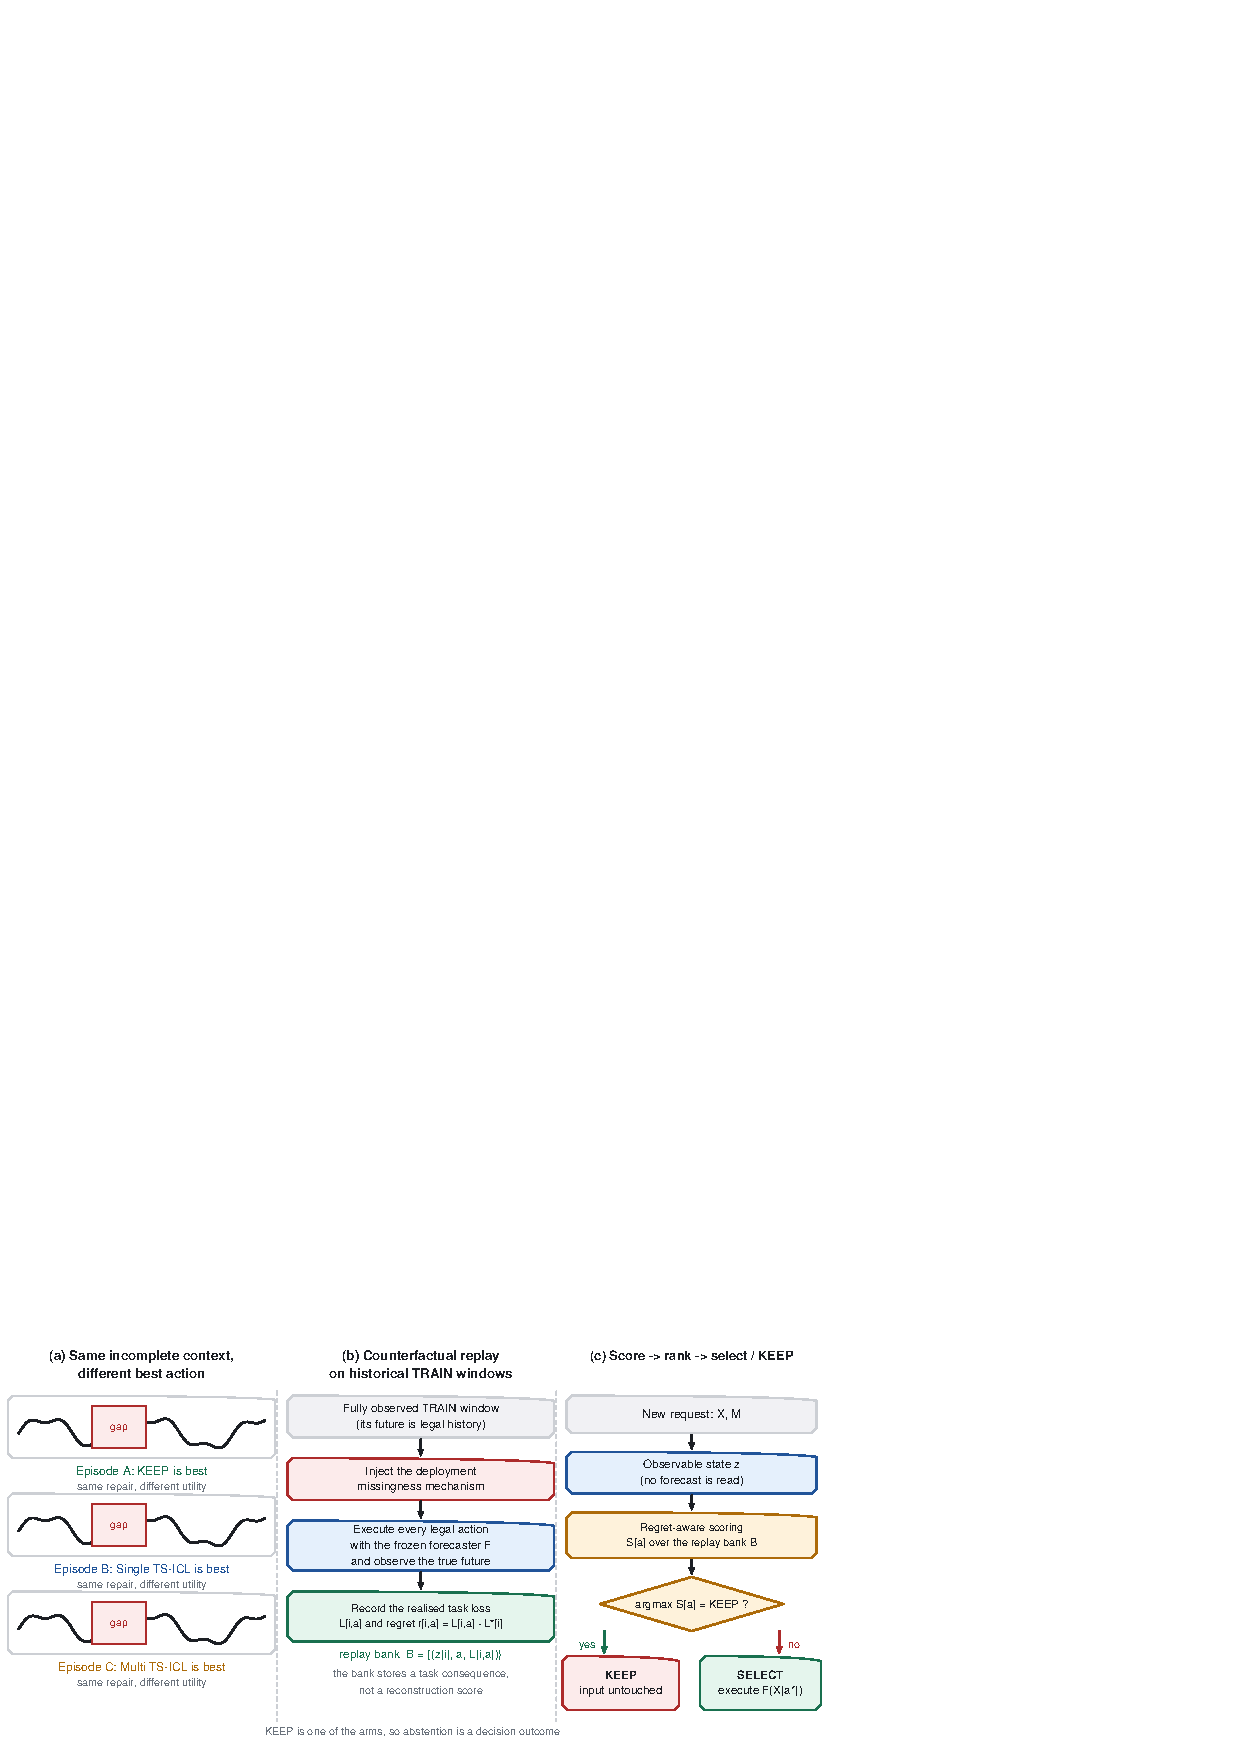
\includegraphics[width=0.64\textwidth]{figure/fig1_selective_governance.pdf}
  \caption{\textbf{(a)}~Share of held-out episodes on which each catalog action is oracle-best.
  No action holds the role often enough for one fixed choice to serve every request.
  \textbf{(b)}~Historical full-action replay on TRAIN. \textbf{(c)}~The online decision, which
  executes an action only when its conservative score is positive.}
  \label{fig:concept}
\end{figure}

% ===========================================================================
\section{Related Work}
\label{sec:related}

\subsection{Incomplete Time-Series Modeling}
\label{sec:related-incomplete}
Three routes handle an incomplete input, and they differ in what they optimise. The first
reconstructs the hidden values and is scored on how close the reconstruction
is~\citep{cao2018brits,tashiro2021csdi,yoon2018gain,du2023saits,park2026t1}. The second builds
a forecaster that reads the missing pattern directly, on the argument that imputing first and
forecasting afterwards accumulates error~\citep{chen2024bitgraph,peng2025s4m,
jang2026channeltokenformer}. These are complete models whose parameters are part of the
contribution. The third replaces the recovery objective with a downstream
one~\citep{wang2024taskoriented,hao2025toivsf,hao2025gimcc,liang2025vida,xu2026srdi}, mostly in
\emph{variable subset forecasting}, where whole variables are absent at inference rather than
positions inside the context.

So the three routes recover the hidden values, train a predictor that tolerates them, or pick
an imputation strategy from corpus-level task performance. \introact{} keeps the predictor fixed
and works at the deployment stage, where the request has arrived, the backbone is frozen, the
future target is unavailable, and the system selects one input version from a finite catalog or
keeps the reference input.

\subsection{Data-Side Adaptation for Frozen \tsfm{}s}
\label{sec:related-dataside}
TATO~\citep{qiu2026tato} shows that a frozen \tsfm{} can be adapted to heterogeneous domains
without parameter updates. It searches a transformation pipeline, including context slicing,
scale normalisation, and outlier correction, and selects the pipeline from historical task
performance. The unit of adaptation is a target domain. TS-ICL~\citep{tsicl2026} is a
foundation model that natively supports imputation, irregular observations, and partially
observed look-back windows. It appears here only as the in-context regression backend of two
catalog actions, so two of the five actions cost one call to a frozen imputation model on top
of the forecasting call (\S\ref{sec:method-deploy}).

The unit of decision is what separates them from \introact{}. TATO selects one transformation
per domain and applies it to every request from that domain. \introact{} selects per request,
and it selects from a closed catalog.

\subsection{Selective Decision Making}
\label{sec:related-selective}
Selective prediction abstains on part of the input to trade coverage for lower
risk~\citep{chow1970optimum,vovk2005algorithmic,geifman2017selective,lei2018distribution}, and
learning to defer routes it to another decision maker~\citep{madras2018predict,
mozannar2020consistent}. Both change who or what produces the answer. Here the same frozen
forecaster answers every request and what is selected is whether the input is modified first.
The decision layer is a supervised local estimation problem. Replay executes every action on
the same window against the same realised future, so the bank holds full action outcomes and no
propensity correction arises, which is what separates it from off-policy
evaluation~\citep{dudik2011doubly,swaminathan2015counterfactual}. Appendix~\ref{app:ope-positioning} states the positioning in
full.

% ===========================================================================
\section{Problem Formulation and Method}
\label{sec:method}

\begin{figure}[t]
  \centering
  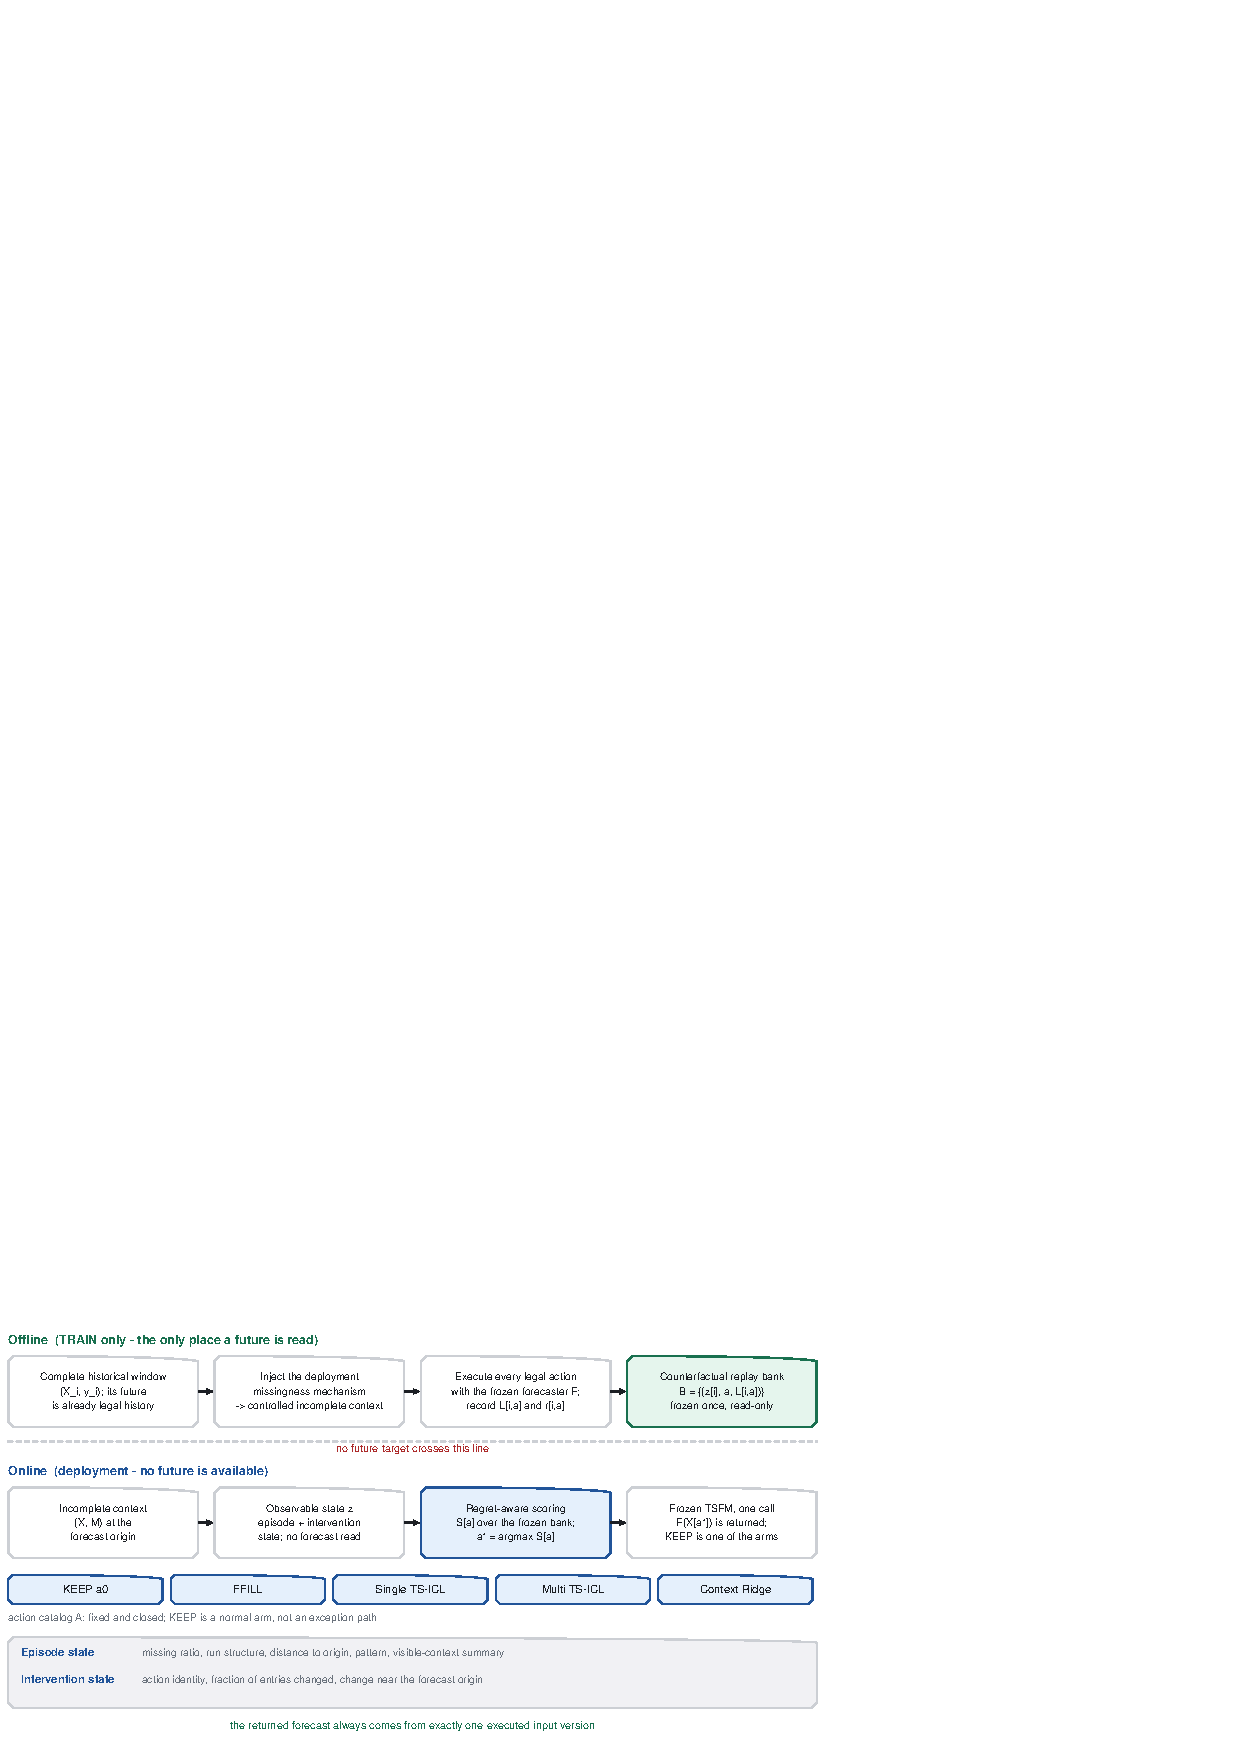
\includegraphics[width=0.48\textwidth]{figure/fig2_introact_architecture.pdf}
  \caption{Architecture of \introact{}. \textbf{Offline}: TRAIN windows become incomplete
  contexts under the registered missingness protocol, every catalog action is executed with the
  frozen forecaster, and the realised utilities populate the replay bank. This is the only place
  a future is read. \textbf{Online}: the reference forecast is computed, an action-conditioned
  state $z_a$ is formed per action and scored against the frozen bank, and one action is
  executed with the same frozen forecaster.}
  \label{fig:arch}
\end{figure}

\subsection{Problem Setup}
\label{sec:method-problem}
Let $X \in \mathbb{R}^{C \times L}$ be the multivariate context at the forecast origin, with
observation mask $M \in \{0,1\}^{C \times L}$, and let $Y \in \mathbb{R}^{C \times H}$ be the
future target, which is never available to the decision procedure. Let $F$ denote the complete
frozen deployment inference pipeline, which takes an input version and returns a forecast
$p = F(X)$ and includes whatever preprocessing the backbone applies internally, so a call to
$F$ is exactly the call the deployed system makes. The reference action hands the incomplete
context to that pipeline unchanged, so what \textsc{Keep} means in practice is whatever
missing-value handling the backbone already performs, which differs between backbone families.
We measure it, and \S\ref{sec:exp-exists} reports how far the two development backbones diverge
on this point.

Let $\calA = \{a_0, a_1, \dots, a_J\}$ be a fixed catalog of admissible interventions, with
$J$ interventions in addition to the reference. Each action $a$ materialises an admissible
input version $X^{a} = T_a(X, M)$. The reference action $a_0$ returns the input unchanged and
corresponds to no external intervention, and $\calA^{+} = \calA \setminus \{a_0\}$ collects
the actions that modify the input. Let $\loss$ be the forecasting loss, defined on the same
normalised scale as the primary evaluation metric so that replay utilities and reported errors
are directly comparable. Utility is measured against the reference, so for a realised target
$Y$,
\begin{equation}
  g_a \;=\; \loss\!\left(F(X^{a_0}),\, Y\right) \;-\; \loss\!\left(F(X^{a}),\, Y\right),
  \label{eq:utility}
\end{equation}
and the task is to choose $a^\star(X, M) \in \calA$ without access to $Y$, while keeping the
number of frozen-backbone calls small.

Three constraints define the deployment protocol. No observation that has arrived and is valid
may be overwritten, so every $X^{a}$ differs from $X^{a_0}$ only at positions where $M = 0$.
The future target is unavailable, so no realised loss is observable at deployment time. The
reference forecast is the only forecast that may be computed before the decision, This is a
call budget, not a claim about what is knowable: a request may spend one
forecasting-backbone call to obtain $p_0 = F(X^{a_0})$, and the forecasts of the remaining
candidates must not be inspected when the action is chosen.

\subsection{Historical Full-Action Replay}
\label{sec:method-replay}
The quantity that decides the action, $g_a$, depends on $Y$ and is not observable online, but it
is computable for a historical window whose target is already part of the available history.
Take such a window $i$, inject the registered missingness protocol to obtain $(X_i, M_i)$,
materialise every action, and execute the frozen pipeline on each version. The realised utility
of action $a$ on window $i$ is
\begin{equation}
  g_{i,a} \;=\; \loss\!\left(F(T_{a_0}(X_i, M_i)),\, y_i\right)
  \;-\; \loss\!\left(F(T_{a}(X_i, M_i)),\, y_i\right).
  \label{eq:replay-gain}
\end{equation}
Both terms are evaluated against the same realised future, so this is a measurement rather
than a model of what the action would have done.

The state recorded with each outcome is action conditioned. For window $i$ and action $a$,
\begin{equation}
  z_{i,a} \;=\; \phi\!\left(X_i,\, M_i,\, X_i^{a},\, p_i^{0}\right),
  \qquad
  p_i^{0} = F(X_i^{a_0}),
  \label{eq:state}
\end{equation}
where $X_i^{a} = T_a(X_i, M_i)$. The state may use the reference forecast $p_i^0$, which the
protocol already permits, and it never uses the forecast of a non-selected candidate. The
replay bank is
\begin{equation}
  \calB \;=\; \bigl\{\, (z_{i,a},\, a,\, g_{i,a}) \,\bigr\},
  \label{eq:replay-bank}
\end{equation}
built once from TRAIN history and then frozen. Deployment reads it and never writes to it.

Two properties of the bank set the scope of the method. A utility measured with one revision
of one model does not describe another, so the bank is built and held per frozen backbone
revision, and serving a new backbone family means rebuilding it. The bank also covers only the
missingness protocol registered in advance, which makes it a discrete grid over patterns and
severities rather than a model of missingness. Retrieval itself is not restricted to a source
or a horizon: the state carries the mask geometry, the visible context and the reference
forecast, which is what the neighbourhood is meant to match on, and restricting retrieval to
the request's own source or horizon costs accuracy on one development backbone while gaining
little on the other (Appendix~\ref{app:replay}).

The step from the bank to a decision rests on one empirical assumption, stated explicitly.
Requests whose action-conditioned states are close in the state space have similar action
utilities, so the utility of an action on a new request can be estimated from the same-action
neighbourhood of its state in the bank. This local transfer assumption is not asserted outside
the registered grid, and the paper makes no claim about behaviour beyond the patterns and
severities that were replayed.

\subsection{Action-Conditioned Local Utility Estimation}
\label{sec:method-scoring}
The estimator is a weighted average of the recorded utilities of the same action on nearby
states, in a fixed standardised feature space. The state $z_a$ of \eqref{eq:state} carries
four groups of features, twenty-two numbers in total. Mask state describes how the request is
incomplete, through the missing fraction, the run structure of the gaps, the distance from the
nearest gap to the forecast origin, and whether other channels are affected. Visible-context
state summarises the observed part of the target channel. Intervention state describes how
$X^{a}$ differs from $X^{a_0}$. Reference-forecast state summarises $p_0 = F(X^{a_0})$.
Appendix~\ref{app:features} is the canonical list, with the window lengths and the
normalisation, which is fitted on the replay bank only.

Retrieval is performed separately for each action. For action $a$, the neighbourhood
$\calN_a$ contains the $k$ bank records whose recorded action is $a$ and whose states are
closest to $z_a$ in standardised Euclidean distance. Each neighbour receives the weight
\begin{equation}
  w_i \;=\; \exp\!\left(-d_i / \tau\right),
  \qquad
  \tau \;=\; \operatorname{median}_{i \in \calN_a} d_i \;+\; \epsilon ,
  \label{eq:weights}
\end{equation}
so the bandwidth is set by the query neighbourhood itself and is not tuned. Taking the median
keeps the effective number of contributing neighbours stable as the local density of the bank
changes, and $\epsilon$ guards the case where every retrieved distance is zero. The local mean
utility, the local dispersion, and the effective sample size are
\begin{equation}
  \hat\mu_a \;=\; \frac{\sum_{i \in \calN_a} w_i\, g_{i,a}}{\sum_{i \in \calN_a} w_i},
  \qquad
  \hat\sigma_a^{2} \;=\; \frac{\sum_{i \in \calN_a} w_i\, (g_{i,a} - \hat\mu_a)^{2}}{\sum_{i \in \calN_a} w_i},
  \qquad
  n_{\mathrm{eff},a} \;=\; \frac{\left(\sum_{i \in \calN_a} w_i\right)^{2}}{\sum_{i \in \calN_a} w_i^{2}} .
  \label{eq:local-moments}
\end{equation}
The neighbourhood size $k$ and the penalty strength $\beta$ of \S\ref{sec:method-decision} are
the only searched quantities, and \S\ref{sec:method-decision} states how they are chosen. The
neighbourhood is defined by distance alone, and no threshold marks a request as outside the
replay support, so the estimator returns a value for every request it receives.
Section~\ref{sec:exp-robust} and Appendix~\ref{app:scope} treat the resulting scope as a
within-grid statement.

\subsection{Conservative Act-or-Keep Decision}
\label{sec:method-decision}
A positive local mean is not sufficient evidence for executing an action, because the
neighbourhood may be small or internally inconsistent. The decision therefore uses the
conservative score
\begin{equation}
  S_a \;=\; \hat\mu_a \;-\; \beta\, \frac{\hat\sigma_a}{\sqrt{n_{\mathrm{eff},a}}},
  \qquad a \in \calA^{+},
  \label{eq:score}
\end{equation}
where $\beta$ is a penalty strength, and
\begin{equation}
  \max_{a \in \calA^{+}} S_a > 0
  \;\Rightarrow\;
  a^{\star} = \arg\max_{a \in \calA^{+}} S_a ,
  \qquad\text{otherwise}\qquad
  a^{\star} = a_0 .
  \label{eq:decision}
\end{equation}
$S_a$ is a heuristic score rather than a calibrated lower bound on $g_a$, it carries no
coverage or risk guarantee~\citep{angelopoulos2024conformal}, and $\beta$ is selected from a
grid rather than read off a sampling distribution. The threshold of zero is not tuned either.
Utility is defined relative to the reference action in \eqref{eq:utility}, so a score at zero
means that the evidence does not distinguish the action from leaving the input unchanged.

The two hyperparameters are selected once per backbone, on the replay bank, by
leave-one-parent-out cross-validation: every bank episode is scored against a bank from which
all records of its own parent have been removed, which makes the cross-validated score a
statement about a request the bank has not seen. The grid is
$k \in \{8, 16, 32, 64\}$ and $\beta \in \{0, 0.5, 1, 1.64\}$. Among the grid points whose
cross-validated conditional harmful rate stays at or below a cap, we take the point with the
lowest cross-validated MASE. The cap is not a free number: it is the conditional harmful rate
of the action with the highest mean realised utility on the same bank, so the constraint says
that choosing per request may not be more harmful, given that it intervenes, than always
applying the strongest single intervention. If no grid point satisfies it the configuration
falls back to the largest penalty strength. The anchor, the cap and the selected pair are
recorded before any evaluation record is scored.

The reference action is always available, so the rule always returns a forecast. It has no way
to detect that a request lies outside the replay support, so it applies to the registered
missingness grid and the results should not be read as out-of-grid generalisation.

\subsection{Deployment Procedure and Cost}
\label{sec:method-deploy}
A request is served in two stages. The first reads the visible context and the mask, executes
the reference action to obtain $p_0$ and the reference-forecast state, materialises the
candidate input versions, and forms the action-conditioned states $z_a$. The second retrieves
the same-action neighbourhoods from the frozen bank, evaluates $S_a$ for every
$a \in \calA^{+}$, executes $a^{\star}$, and returns the resulting forecast, which is the
reference forecast when $a^{\star} = a_0$.

A request costs one forecasting-backbone call for the reference action plus one more if an
intervention is executed, and the returned forecast is always one call of the unchanged $F$ on
one executed input version. Two of the four interventions build their candidate by calling a
frozen in-context imputation model, which is paid before the decision.
Appendix~\ref{app:calls} keeps the one-off bank construction, candidate materialisation, the
backbone call and retrieval overhead in separate columns.

% ===========================================================================
\section{Experiments}
\label{sec:exp}

\subsection{Experimental Setup}
\label{sec:exp-setup}
The main matrix covers eight public forecasting sources (ETTh1, ETTh2, ETTm1, ETTm2,
Electricity, Exchange, Traffic, and Weather) and three frozen \tsfm{} families:
Chronos-Bolt~\citep{chronosbolt2025}, TimesFM-2.5~\citep{das2024timesfm}, and
Chronos-2~\citep{chronos2_2025}. The first two are used for method development. Chronos-2
enters only after the configuration is frozen, with the identical algorithm and the same
selection rule applied to a replay bank rebuilt with Chronos-2 itself, so what transfers is the
procedure and not the bank.
Context length is $L = 512$ and the main horizons are $H \in \{96, 192\}$. Four deterministic
missingness patterns are frozen before any method runs, and every mask is derived by a
deterministic hash of source, parent, origin, horizon, pattern, and protocol seed. The main
comparison uses $10\%$ severity, and \S\ref{sec:exp-robust} adds $30\%$ and $50\%$ inside the
same registered grid. Appendix~\ref{app:data-protocol} defines the patterns, the derivation
rule, and the metric denominators.

The catalog is fixed at five admissible actions with \textsc{Keep} as the reference $a_0$, and
a complete and valid input is always mapped to \textsc{Keep}. Appendix~\ref{app:catalog}
defines each action and the status rules for unsupported, aliased, or failed executions.

The comparison is fixed in advance. Three controls establish what a per-request decision has to
beat. \textsc{Native Keep} never intervenes and is the reference every other row is measured
against. \textsc{Best Fixed} applies to every request the single catalog action with the
highest mean realised utility on the replay bank, which makes it the strongest policy that
ignores the request. \textbf{R2-CART} is the simple learned selector inherited from the
previous development cycle: one depth-three classification tree per action over the same state
features, each asking whether that action beats the reference, executing the most confident
action when its probability exceeds one half. Two published methods compose with a frozen
backbone and are reported in full: SAITS~\citep{du2023saits,du2023pypots} is the
reconstruction baseline, trained per source on the same TRAIN windows under the same
missingness protocol, and TATO~\citep{qiu2026tato} is the data-side adaptation baseline, whose
transformation pipeline is searched per source against the realised futures of the same TRAIN
windows the replay bank is built from, so neither method is given evidence the other lacks. A
\emph{Catalog Oracle} that reads the future target is reported as a diagnostic and excluded
from all ranks.
The severity sweep of \S\ref{sec:exp-robust} keeps the same frozen configuration and the same
roster. Appendix~\ref{app:datasets} documents the roster and the per-source tables, and
Appendix~\ref{app:baseline-availability} records which published methods have a public
implementation that admits our protocol and which do not.

Each source is split chronologically at three quarters of its rows, the earlier part TRAIN and
the later part TEST, and the last TRAIN window of each source is dropped so the gap exceeds the
$L + H$ purge everywhere. TRAIN is split by origin time into the replay bank and a TRAIN-eval
block used once as an internal acceptance check. All design, hyperparameter selection, feature
normalisation and baseline fitting use TRAIN only, and every reported table is computed once on
TEST after the configuration is frozen. MASE~\citep{hyndman2006mase} is the primary metric and
RMSSE the secondary one, aggregated source-macro with the parent as the statistical unit and
paired cluster bootstrap intervals. Appendices \ref{app:splits},
\ref{app:metric-conventions} and \ref{app:diagnostic-conventions} hold the split boundaries,
the metric and statistics conventions, and the diagnostic counting rules.

\subsection{Does Selective Intervention Need to Exist?}
\label{sec:exp-exists}
Both statistics below are diagnostics computed on TEST after the configuration is frozen and
are used for no selection. The first premise is that the best action varies across requests.
For each episode the oracle-best action is the minimiser of the realised loss over the catalog,
and Figure~\ref{fig:concept}(a) shows how often each action takes that role. No action is oracle-best on more than 24\% of the episodes and none on fewer than 15\%, with the untouched input best on 24\% of them. The catalog oracle reaches 1.307 against 1.576 for the untouched input, so the catalog carries 0.269 MASE of achievable improvement. One fixed intervention applied everywhere recovers 51\% of that improvement, and the rest is what a per-request decision has to find.

Every intervention helps on some requests and hurts on others. The weakest, forward fill, improves the forecast on 48\% of the episodes where it applies and the strongest, context ridge, on 58\%, so none is safe to apply unconditionally and none is safe to drop.

The second premise is that reconstruction quality does not tell a deployment which repair to
run. All four interventions estimate the hidden positions explicitly and the mask is synthetic,
so both rankings exist for the same episode, and ranking inside an episode keeps sources of
different scale apart. The repair with the lowest reconstruction error is also the one with the highest realised utility on 21\% of the episodes, against 20\% for picking at random among the same repairs, 44\% of the ordered pairs disagree, and the mean within-episode rank correlation between the two criteria is 0.13. On average multivariate in-context regression recovers the hidden values most accurately while context ridge helps the forecast most, so the two criteria do not even agree on the corpus. Figure~\ref{fig:why-selective}(a) shows it and
Appendix~\ref{app:recutils} reports it per action. \introact{} is not in this ranking, because
it returns a forecast from an executed input rather than a reconstruction.

\begin{figure}[t]
  \centering
  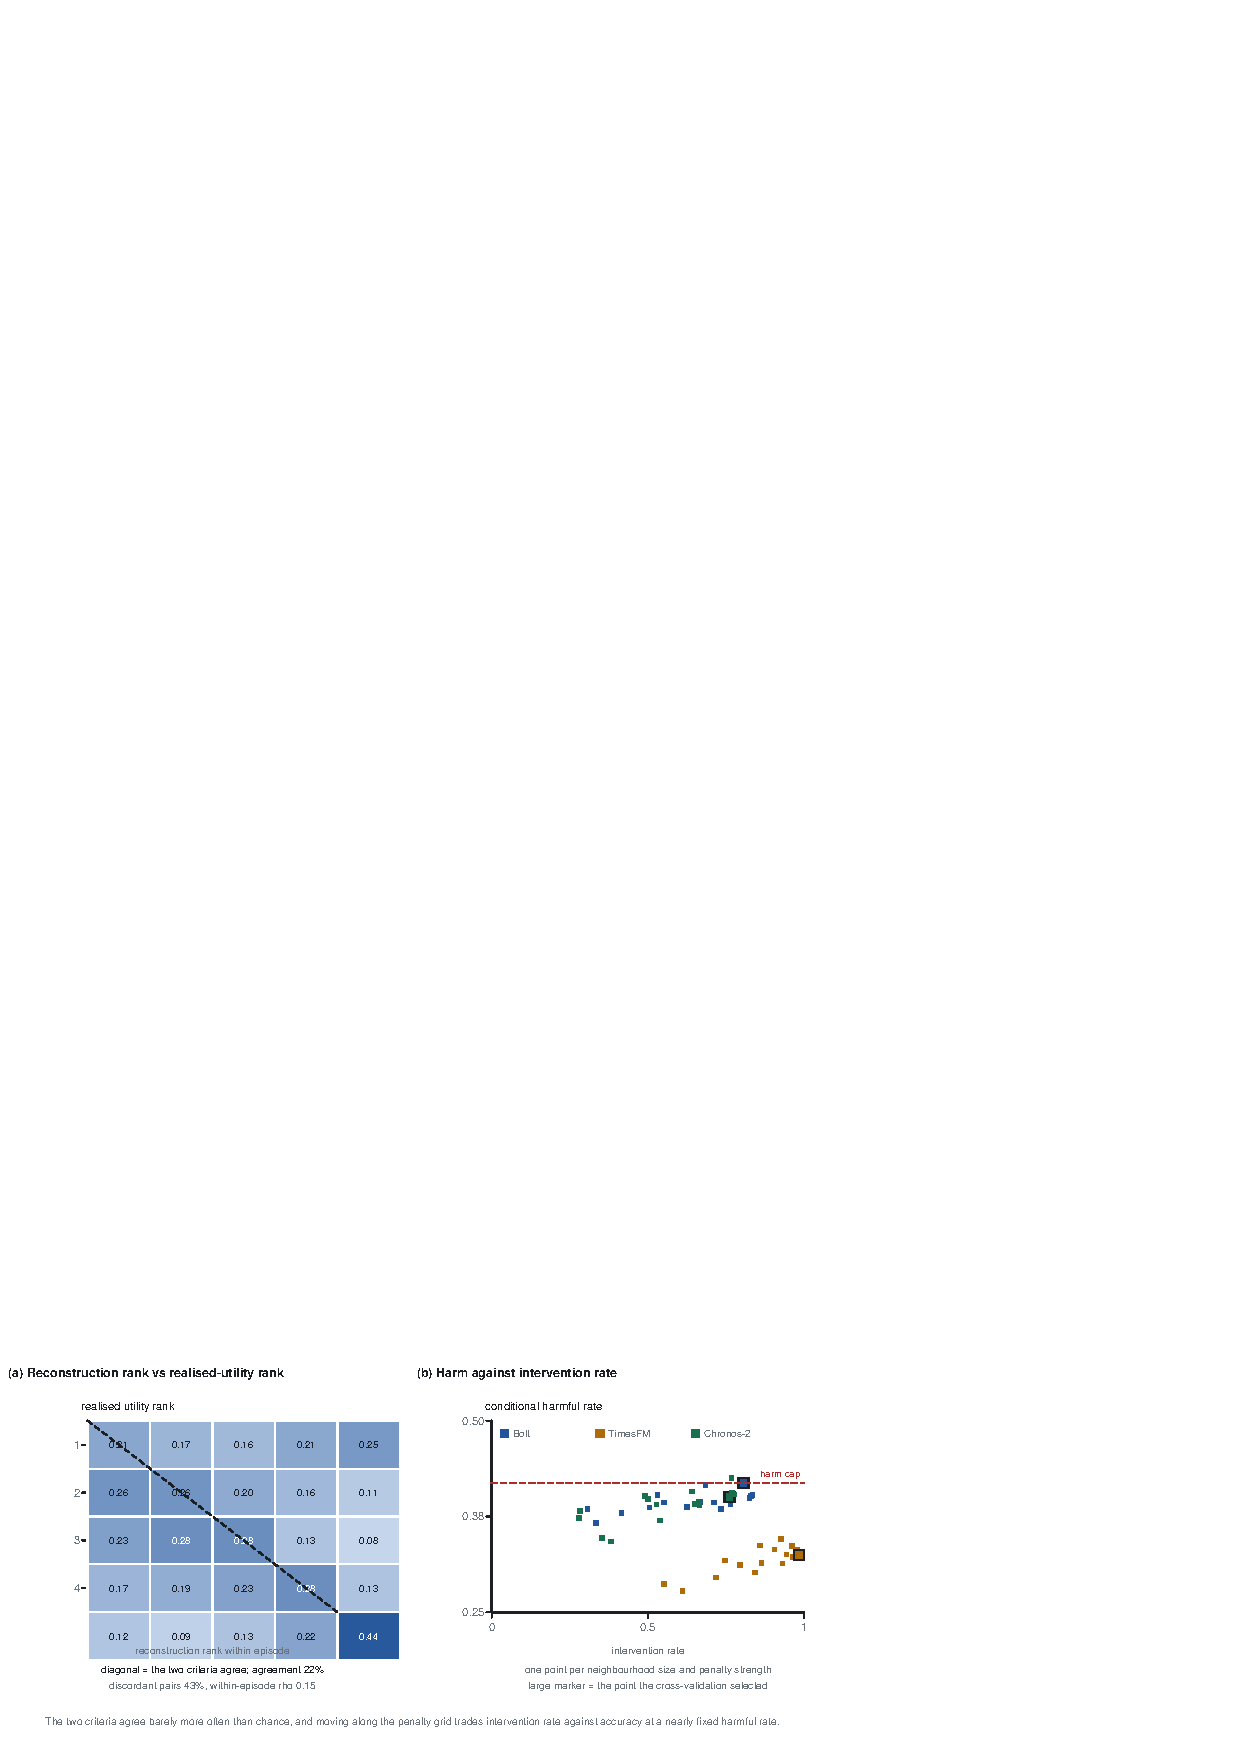
\includegraphics[width=0.62\textwidth]{figure/fig3_why_selective.pdf}
  \caption{\textbf{(a)}~Joint distribution of the within-episode reconstruction rank and the
  within-episode realised-utility rank over the four catalog interventions and SAITS,
  row-normalised over
  the held-out episodes of all three backbones. Off-diagonal mass is episodes on which the more
  accurate reconstruction is not the more useful intervention. \textbf{(b)}~Cross-validated
  conditional harmful rate against intervention rate over the neighbourhood and penalty grid,
  one point per grid cell per backbone, with the selected point enlarged and the cap marked.}
  \label{fig:why-selective}
\end{figure}

Appendix~\ref{app:opportunity} breaks the same episodes down by how much improvement was
available.

\subsection{Main Comparison}
\label{sec:exp-main}
\emph{Does deciding per request beat doing nothing, applying one repair everywhere, and
learning a simple selector, across sources and frozen \tsfm{} backbones?}

Table~\ref{tab:main} reports the main comparison at $10\%$ severity over all eight sources,
three backbones, two horizons, and four patterns. \introact{} reaches 1.447 source-macro MASE against 1.576 for the untouched input, 1.438 for the best fixed intervention and 1.456 for the simple selector, and against the published baselines at SAITS 1.696, TATO 1.689. It improves on the untouched input on every backbone.
Against the untouched input the paired difference is Bolt -0.0957 [-0.1525, -0.0397], TimesFM -0.1554 [-0.2055, -0.1050], Chronos-2 -0.1370 [-0.1625, -0.1124], and every interval excludes zero. Against the best fixed intervention the interval excludes zero on Bolt. It is the lowest deployable row on Bolt and TimesFM, and on Chronos-2 one fixed repair reaches a lower macro average, which \S\ref{sec:exp-robust} returns to. The deployable rows span 1.438 to 1.696 and the catalog oracle sits at 1.307, so the room to recover is bounded and the gaps between rows are a visible part of it. Both published baselines repair or transform every incomplete request, and SAITS ends at 1.696 and TATO ends at 1.689, above the 1.576 of leaving the input alone. The loss is concentrated rather than uniform, with SAITS below it on 18 of 24 source and backbone cells, TATO below it on 5 of 24 source and backbone cells, so what costs a fixed repair its average is the minority of cells on which it is badly wrong, and that is the failure a per-request rule can avoid. Against the simple selector no interval excludes zero, so accuracy alone does not separate the two and what does is in Table~
ef{tab:harm}.
Average rank over the evaluation cells is Bolt 4.17, TimesFM 3.83, Chronos-2 4.01, against Bolt 4.17, TimesFM 3.82, Chronos-2 4.01 for the best row on each. Per-source MASE, MAE, and RMSE are in Appendix~\ref{app:datasets}, and
deployment cost is reported separately in Appendix~\ref{app:calls}.

\begin{table}[t]
  \caption{Main comparison on TEST at $10\%$ missingness. MASE and RMSSE are source-macro
  averaged and lower is better everywhere. Every row composes with the same frozen backbone and
  therefore shares one reference contract. \best{Bold} marks the best deployable method and
  \second{underline} the second best. The oracle row reads the future target for diagnosis only
  and is excluded from the ranks. Chronos-2 is a held-out backbone whose configuration is
  selected by the same frozen procedure on its own replay bank and is not retuned.}
  \label{tab:main}
  \centering
  \small
  \setlength{\tabcolsep}{3.5pt}
\resizebox{\textwidth}{!}{\begin{tabular}{llccccc c}
    \toprule
    Method & Type & Bolt MASE $\downarrow$ & TimesFM MASE $\downarrow$
           & Chronos-2 MASE $\downarrow$ & Overall MASE $\downarrow$
           & Overall RMSSE $\downarrow$ & Avg.\ rank $\downarrow$ \\
    \midrule
    Native KEEP        & Frozen \tsfm{}          & 1.466   & 1.682   & 1.579   & 1.576   & 1.325   & 5.99 \\
    Best Fixed         & Fixed policy            & 1.386     & 1.576     & \best{1.353}     & \best{1.438}     & \best{1.233}     & \second{4.42} \\
    R2-CART            & Simple selector         & \second{1.375}     & \second{1.558}     & \second{1.435}     & 1.456     & 1.244     & 4.80 \\
    SAITS              & Reconstruction          & 1.673  & 1.739  & 1.676  & 1.696  & 1.414  & 5.76 \\
    TATO               & Data-side adaptation    & 1.742   & 1.621   & 1.704   & 1.689   & 1.375   & 7.20 \\
    \midrule
    \rowcolor{bestgray}\introact{} & Frozen governance & \best{1.371} & \best{1.527} & 1.442 & \second{1.447} & \second{1.239} & \best{4.00} \\
    \midrule
    Catalog Oracle     & Diagnostic              & \oracle{1.262} & \oracle{1.417} & \oracle{1.241} & \oracle{1.307} & \oracle{1.129} & \oracle{--} \\
    \bottomrule
  \end{tabular}}
\end{table}

\subsection{Does Selective Replay Reduce Harm?}
\label{sec:exp-harm}
\emph{Is the gain produced by choosing better interventions, or by intervening less often?}

Table~\ref{tab:harm} reports the selective-governance diagnostics at the default operating
point. An intervention is harmful when it increases the realised loss relative to leaving the
input unchanged, so the conditional harmful rate is conditioned on the requests where an
intervention was executed and must be read together with the intervention rate, because a
method that intervenes on almost nothing can report a low conditional rate without
contributing anything. Beneficial precision is the share of executed interventions that reduced
the loss, and missed opportunity is the share of episodes with a positive oracle opportunity on
which nothing was executed. \introact{} executes an intervention on 83\% of the requests, so its accuracy is not bought by staying still, while the published baselines repair or transform every incomplete request by construction, so their intervention rate is one. Conditional on intervening it is harmful on 44.2\% of those requests against 42.7\% for the fixed intervention and 43.9\% for the simple selector. Harmful loss, which weights each harmful intervention by the loss it added, is 0.0451, against the best fixed intervention 0.0536, the simple selector 0.0505, SAITS 0.1065, TATO 0.2937. The selective rule is therefore both more accurate and cheaper when wrong.
Beneficial precision is 55.8\%. and missed opportunity is 17.8\%, which is what the reference option costs.

Figure~\ref{fig:why-selective}(b) traces the trade-off over the score grid by post-processing
the stored scores on TEST, with no threshold selected on TEST.
Appendix~\ref{app:governance-fig} reports the curve cell by cell. Raising the penalty strength walks the operating point down the curve, trading accuracy for a lower intervention rate while the conditional harmful rate moves little, so the rate at which an executed intervention hurts is a property of the catalog rather than of how cautious the rule is.

\begin{table}[t]
  \caption{Selective-governance diagnostics at the default operating point, $10\%$ severity.
  Intervention rate is the share of requests on which a non-reference action was executed.
  Conditional harmful rate is the share of executed interventions that increased the realised
  loss relative to \textsc{Keep}, and harmful loss is the mean increase over those requests.
  Beneficial precision is the share of executed interventions that reduced the loss, and missed
  opportunity is the share of positive-opportunity episodes on which nothing was executed.}
  \label{tab:harm}
  \centering
  \small
  \setlength{\tabcolsep}{3.5pt}
\resizebox{\textwidth}{!}{\begin{tabular}{lcccccc}
    \toprule
    Method & MASE $\downarrow$ & Intervention rate & Conditional HIR $\downarrow$ & Harmful loss $\downarrow$ & Beneficial precision $\uparrow$ & Missed opportunity $\downarrow$ \\
    \midrule
    Native KEEP        & 1.576   & 0.0\%   & 0.0\%   & 0.0000   & ---   & 100.0\% \\
    Best Fixed         & 1.438     & 83.3\%     & 42.7\%     & 0.0536     & 57.3\%     & 15.3\% \\
    R2-CART            & 1.456     & 96.8\%     & 43.9\%     & 0.0505     & 56.1\%     & 3.1\% \\
    SAITS              & 1.696     & 100.0\%     & 45.4\%     & 0.1065     & 54.6\%     & 0.0\% \\
    TATO               & 1.689   & 100.0\%   & 59.2\%   & 0.2937   & 40.8\%   & 0.0\% \\
    \midrule
    \rowcolor{bestgray}\introact{} & 1.447 & 82.6\% & 44.2\% & 0.0451 & 55.8\% & 17.8\% \\
    \bottomrule
  \end{tabular}}
  \vspace{-2pt}
  {\footnotesize A method that always returns a repaired input intervenes on every incomplete
  request by construction, so its intervention rate is one and its conditional harmful rate is
  unconditional. \textsc{Context Ridge} is not admissible on the shared-block pattern, so a
  fixed policy that selects it intervenes on fewer than all requests.}
\end{table}

\subsection{Robustness and Transfer}
\label{sec:exp-robust}
\emph{Does one frozen configuration remain useful as missingness becomes more severe, and does
it carry over to a backbone family that was not used during development?}

Severities are $10\%$, $30\%$, and $50\%$, crossed with the four patterns and the three
backbones, and no method is retuned between levels. The levels lie inside the registered grid
that the replay bank samples from, so this is a within-grid robustness check and not an
unseen-severity stress test. and the roster is the one of Table~\ref{tab:main}.
Table~\ref{tab:robust} in Appendix~\ref{app:severity-full} reports the severity trend and the worst pattern cell, and the
held-out backbone is the Chronos-2 column of Table~\ref{tab:main}.
Against the untouched input the frozen configuration holds at every level: 10\% 1.447 against 1.576, 30\% 1.475 against 1.794, 50\% 1.561 against 1.875. The ordering between the deployable rows does change with severity: at 10\% the best fixed intervention reaches 1.438, at 30\% the simple selector reaches 1.469. The configuration is frozen on a bank that mixes the three levels, so the sweep shows how far one operating point carries rather than what a per-level tuning could reach. On the held-out family the frozen procedure improves on the untouched input, 1.442 against 1.579 with a paired interval that excludes zero, it has the best average rank of the deployable rows at 4.01, and the lowest macro average there belongs to the best fixed intervention at 1.353.
Appendix~\ref{app:severity-full} holds the complete per-severity tables and
Appendix~\ref{app:pattern} holds the per-pattern tables.
\subsection{Ablation and Cost}
\label{sec:exp-ablation}
\emph{Which component carries the gain, and what does a request cost?}

Every ablation reuses the same catalog prediction cache, so the rows are recomputed selector
variants rather than new forecasting runs. A1 scores each action by its global mean utility
instead of by its neighbourhood, A2 and A3 drop the intervention and the reference-forecast
block of the state, A4 removes the reference option so that an action runs on every request,
and A5 replaces the local estimate with a per-action linear utility predictor over the same
features. Appendix~\ref{app:ablation-details} gives the exact definitions.
Table~\ref{tab:ablation} reports accuracy, harm, and cost together. Two parts of the design carry the result, and the state blocks matter less than either. Scoring an action by its global mean utility instead of its neighbourhood costs -0.0150 [-0.0296, -0.0004] and drives the intervention rate to 100\%, which is what a corpus-level answer to a per-request question looks like. Dropping the intervention block of the state changes accuracy by -0.0006 [-0.0038, +0.0029]. Dropping the reference-forecast block changes it by +0.0068 [-0.0083, +0.0216], so neither state block is load bearing on its own.
Removing the reference option and executing the best-scoring action on every request changes accuracy by +0.0076 [-0.0004, +0.0167] while raising harmful loss from 0.0451 to 0.0519, so keeping the input is what lets the method intervene on 17\% fewer requests without paying for it in accuracy. Replacing retrieval by a per-action linear utility predictor over the same features costs -0.0259 [-0.0440, -0.0081], the largest gap in the table and the clearest sign that the local estimate is doing the work. A request costs 1.83 forecasting-backbone calls on average.

\begin{table}[t]
  \caption{Core ablation and cost at $10\%$ severity, on the held-out evaluation set. Every
  row reads the same catalog prediction cache, so the rows differ only in how the stored
  utilities are summarised and thresholded. Calls counts forecasting-backbone calls per
  request and equals one plus the intervention rate; candidate materialisation is reported
  separately in Appendix~\ref{app:calls}.}
  \label{tab:ablation}
  \centering
  \small
  \setlength{\tabcolsep}{3.5pt}
\resizebox{\textwidth}{!}{\begin{tabular}{lccccc}
    \toprule
    Variant & MASE $\downarrow$ & Intervention rate & Conditional HIR $\downarrow$ & Harmful loss $\downarrow$ & Calls $\downarrow$ \\
    \midrule
    Full \introact{}          & 1.447   & 82.6\%   & 44.2\%   & 0.0451   & 1.83 \\
    A1 Global utility          & 1.462     & 100.0\%     & 43.9\%     & 0.0642     & 2.00 \\
    A2 w/o intervention state  & 1.446     & 82.4\%     & 43.8\%     & 0.0460     & 1.82 \\
    A3 w/o reference-forecast state & 1.426 & 84.8\%     & 42.6\%     & 0.0426     & 1.85 \\
    A4 Always act              & 1.439     & 100.0\%     & 44.6\%     & 0.0519     & 2.00 \\
    A5 Parametric utility predictor & 1.462 & 87.2\%    & 44.0\%     & 0.0574     & 1.87 \\
    \midrule
    \bottomrule
  \end{tabular}}
\end{table}

% ===========================================================================
\section{Conclusion}
\label{sec:conclusion}
We studied incomplete-input handling for frozen \tsfm{}s as a per-request decision over a fixed
catalog of admissible interventions. The realised utility of an intervention is not observable
at forecast time, and reconstruction quality turns out to be close to uninformative about it,
so \introact{} reads the answer off history: it replays TRAIN windows as pseudo-deployments,
executes every catalog action with the frozen forecaster, and stores what each action did.

The evaluation supports three claims. Deciding per request lowers source-macro MASE from 1.576 to 1.447, and it has the best average rank of the deployable rows on every backbone. The reference action is returned on 17\% of requests, which lowers harmful loss relative to executing an action every time without costing accuracy. The same procedure, with its two hyperparameters chosen by the same cross-validation rule on the backbone's own replay bank, still improves on the untouched input and still ranks first among the deployable rows on a backbone family that took no part in method design, without reaching the lowest average there.
The evidence also has a clear boundary. All missingness here comes from controlled deletion
under a registered protocol, the replay bank covers only the patterns and severities that were
replayed, and the method cannot detect that a request lies outside that grid. The results
therefore support selective intervention under the evaluated controlled-missingness protocols
and frozen backbones, and generalisation to unseen mechanisms and to naturally incomplete
streams remains open. What the method needs is not a better imputer but a record of what the available imputers already did to the model that will be asked to forecast.

\subsubsection*{AI use statement}
We used generative AI tools to assist with literature review, prose editing, code drafting and
refactoring, figure preparation, and discussion of methodological and experimental choices.
All methodological decisions, experimental protocols, code changes, and reported results were
reviewed and approved by the authors. Generative AI was not used to fabricate or alter
experimental measurements, and no numerical result in this paper was generated by a language
model. Every reported number is produced by the recorded experiment pipeline described in
Appendix~\ref{app:reprodetails} and is traceable to a stored artefact. We take responsibility
for the final content of this work, including its text, claims, and artefacts.

\subsubsection*{Ethics statement}
This work studies input governance for frozen forecasting models on public benchmark datasets.
It does not involve human subjects, personal data, or deployment decisions with direct
societal consequences. We impose an integrity constraint under which an admissible
intervention cannot overwrite an observation that is marked as valid and available, because
silently replacing a real measurement would be a data integrity problem regardless of its
forecasting effect. We do not claim safety, robustness, or generality beyond the measured
conditions.

\subsubsection*{Reproducibility statement}
We provide the complete experimental protocol, the final TRAIN and TEST split with the
purging rule, the missingness generation procedure, the intervention catalog, the state
feature definitions, the hyperparameter search spaces, the failure policy, and the statistical
analysis in Appendix~\ref{app:data-protocol} and Appendix~\ref{app:splits}.
Appendix~\ref{app:reprodetails} specifies the result-record schema and the traceability checks.
All reported tables are generated from retained raw predictions and versioned configurations.

\bibliography{references}
\bibliographystyle{iclr2027_conference}

% ===========================================================================
% ===========================================================================
% 附录（由正文下沉 + 完整化）。所有未运行数字一律 \ph{KEY}，禁止编造。
% ===========================================================================



\appendix

\newpage



\section*{Appendix map}
\label{app:map}
Table~\ref{tab:app-map} lists what each appendix section contains. The appendix is organised
by evidence type rather than by individual analysis, and a final unnumbered section holds
exploratory material that supports no claim in the main text.

\begin{table}[h]
  \caption{Appendix map. Sections are lettered in order of appearance. The final
  supplementary section is unnumbered and holds no load-bearing evidence.}
  \label{tab:app-map}
  \centering
  \small
  \setlength{\tabcolsep}{4pt}
\resizebox{\textwidth}{!}{\begin{tabular}{lll}
    \toprule
    Section & Contents & Question it answers \\
    \midrule
    A. Protocol and method details & final TRAIN and TEST split with purging, scope and assumptions, the action catalog, the state feature definitions, the registered missingness patterns, the metric conventions, the diagnostic counting rules, the complete-input contract & what exactly was fixed before the evaluation ran, and which claims are out of scope? \\
    B. Full per-source and per-pattern results & per-source tables for every method, opportunity strata, per-pattern tables, extended comparison & does the aggregate hold source by source, stratum by stratum, and pattern by pattern? \\
    C. Full severity results & $10/30/50\%$ tables and the severity trend & does one frozen configuration hold across the registered severity grid? \\
    D. Reconstruction and utility diagnostics & within-episode rank comparison over the catalog, governance diagnostics & is reconstruction quality a usable substitute for forecasting utility? \\
    E. Ablations and stability & the full ablation vector, the $k$ and $\beta$ gate grid, and mask-realisation stability & which component carries the gain, and is the result an artefact of one mask? \\
    F. Cost, failures, and memory & latency, call counts, candidate materialisation, failures, timeouts, cold start & what does a request actually cost? \\
    G. Reproducibility and artefact schema & record schema, revisions, seeds, environment, manifests & can every reported number be traced back to a stored artefact? \\
    Supplementary (unnumbered) & the preceding development cycle & what was tried and rejected before the present formulation? \\
    \bottomrule
  \end{tabular}}
\end{table}



\section{Protocol and Method Details}
\label{app:protocol}
\subsection{Scope and Assumptions}
\label{app:scope}
This section states what the replay bank is, what it is not, and which claims the paper
therefore does and does not make.

The bank is a discrete grid over four patterns, three severities, and the registered sources,
and it is not a continuous model of missingness. If a request falls outside that grid, which
includes a different missingness mechanism, a different missing-rate regime, or an
unrepresented source family, the estimator still returns a score, but the retrieved
historical utilities need not transfer. The method has no guarantee outside the registered
replay support, because the neighbourhood is defined by distance alone and no threshold marks
a request as unsupported. We therefore read \S\ref{sec:exp-robust} as a within-grid check
rather than as out-of-grid generalisation, and results in this paper should not be interpreted
as out-of-grid generalisation.

Three further assumptions are worth stating explicitly. First, the action catalog is closed and
given. We do not search for new interventions, and a wider catalog would change every number
in this paper without changing the decision problem. Second, the missingness mechanism that
deployment encounters is assumed to be the one that the replay injects. A request produced by
a different mechanism is handled by the same estimator but lies outside the scope of the
reported results. Third, the frozen forecaster is assumed deterministic and revision pinned.
Every replay record is tied to the exact model revision that produced it, and a model update
invalidates the bank rather than silently degrading it.

Four claims are therefore not made anywhere in this paper. We do not claim out-of-grid or
out-of-distribution missingness generalisation. We do not claim that the method can detect
that historical evidence is insufficient. We do not claim any coverage or risk-control
guarantee for the conservative score. We do not claim that the results extend to naturally
incomplete deployment streams, since every missingness realisation in the main matrix comes
from controlled deletion under a registered protocol.


\subsection{Full Method Details}
\label{app:method-details}
This section expands \S\ref{sec:method} with the closed intervention catalog, the canonical
definition of the state features, and the relation of the decision layer to off-policy
evaluation and selective prediction. The state features are defined here once, and the main
text refers to this section rather than restating them.

\subsubsection{Intervention Catalog}
\label{app:catalog}
Table~\ref{tab:app-catalog} defines the five admissible actions. The catalog is closed, so no
action outside this set is ever executed, and no action may overwrite an observation that has
arrived and is valid.

\begin{table}[h]
  \caption{The five admissible interventions. Observed entries are the entries that are
  present and valid in the reference input $X^{a_0}$, and an action that modified them would
  violate the integrity constraint of \S\ref{sec:method-problem}.}
  \label{tab:app-catalog}
  \centering
  \small
  \setlength{\tabcolsep}{4pt}
\resizebox{\textwidth}{!}{\begin{tabular}{llcc}
    \toprule
    Action & Input version produced & May modify observed entries? & Extra backbone calls \\
    \midrule
    \textsc{Keep} $a_0$   & the incomplete context, unchanged & reference action & 0 \\
    \textsc{Ffill}        & forward-fill from the last valid value & no & 1 \\
    \textsc{Single TS-ICL}& univariate in-context regression on the target channel & no & 1 \\
    \textsc{Multi TS-ICL} & multivariate in-context regression using visible channels & no & 1 \\
    \textsc{Context Ridge}& ridge reconstruction from the visible context & no & 1 \\
    \bottomrule
  \end{tabular}}
\end{table}

A complete and valid input is always mapped to \textsc{Keep} and the reference forecast is
returned unchanged. Unsupported, aliased, and failed actions are recorded with an explicit
status, and they are never counted as successes. The required behaviour of the system in each
input regime is listed in \S\ref{app:contract}.

\subsubsection{State Features}
\label{app:features}
The state is action conditioned and is written $z_a$ for action $a$, with
\begin{equation}
  z_a \;=\; \phi\!\left(X,\, M,\, X^{a},\, p_0\right),
  \qquad p_0 = F(X^{a_0}) .
  \label{eq:app-state}
\end{equation}
It contains no future target information. It uses the reference forecast $p_0$, which the
call budget of \S\ref{sec:method-problem} already permits, and it never uses the forecast of a
non-selected candidate. Table~\ref{tab:app-features} is the canonical definition of the four
groups, including the window length, the channel aggregation, and the missing-value handling
of each feature. Continuous features are standardised with statistics fitted on the replay
bank only, and the normalisation is frozen with the rest of the configuration.

\begin{table}[h]
  \caption{The action-conditioned state, as implemented. It has 22 dimensions: six describing
  the mask, six describing the visible context, five describing the candidate intervention and
  five describing the reference forecast. Every feature is computable from the request and the
  reference forecast alone. The target channel is the forecast channel, and the only place the
  other channels enter is the shared indicator. Features are divided by the robust scale $s$ of
  the visible context where they carry a unit, and the state is then standardised with the mean
  and standard deviation of the replay bank before distances are taken.}
  \label{tab:app-features}
  \centering
  \small
  \setlength{\tabcolsep}{4pt}
\resizebox{\textwidth}{!}{\begin{tabular}{@{}l p{0.22\textwidth} p{0.42\textwidth} p{0.16\textwidth}@{}}
    \toprule
    Group & Feature & Definition & Scaling \\
    \midrule
    Mask state, 6 & missing ratio & share of target-channel positions with $M = 0$ & scale free \\
     & longest run & longest run of consecutive missing positions, as a share of $L$ & scale free \\
     & number of runs & count of maximal missing runs, divided by $L$ & scale free \\
     & distance to origin & steps from the end of the last missing run to the forecast origin, divided by $L$ & scale free \\
     & shared indicator & one if any other channel is also missing & binary \\
     & tail indicator & one if the last context position is missing & binary \\
    \midrule
    Visible-context state, 6 & robust scale $s$ & median over eight blocks of the interquartile range of the visible target values & the unit of the other context features \\
     & local trend & least-squares slope over the visible positions, divided by $s$ & scale free \\
     & lag-one autocorrelation & autocorrelation of the gap-interpolated target at lag one & scale free \\
     & seasonal autocorrelation & the same at the registered seasonal period $m$ & scale free \\
     & recent level shift & absolute difference between the means of the last and the preceding $W = 32$ steps, divided by $s$ & scale free \\
     & recent volatility & standard deviation of the first differences over the last $W$ steps, divided by $s$ & scale free \\
    \midrule
    Intervention state, 5, per action $a$ & mean absolute change & mean of $|X^{a} - X^{a_0}|$ over the context, divided by $s$ & scale free \\
     & maximum change & largest absolute difference, divided by $s$ & scale free \\
     & changed fraction & share of positions where $X^{a}$ differs from $X^{a_0}$ & scale free \\
     & change trend & least-squares slope of the difference over the changed positions, divided by $s$ & scale free \\
     & change near origin & mean absolute difference over the last $W$ steps, divided by $s$ & scale free \\
    \midrule
    Reference-forecast state, 5 & forecast level & mean of $p_0$ over the horizon, divided by $s$ & scale free \\
     & forecast range & range of $p_0$ over the horizon, divided by $s$ & scale free \\
     & forecast trend & least-squares slope of $p_0$, divided by $s$ & scale free \\
     & first-step jump & first step of $p_0$ minus the last visible value, divided by $s$ & scale free \\
     & roughness & mean absolute first difference of $p_0$, divided by $s$ & scale free \\
    \bottomrule
  \end{tabular}}
\end{table}

\subsubsection{Relation to Off-Policy Evaluation and Selective Prediction}
\label{app:ope-positioning}
The decision layer is related to conservative policy selection in contextual
bandits~\citep{abbasiyadkori2011improved,lattimore2020bandit} and to off-policy
evaluation~\citep{strehl2010learning,dudik2011doubly,swaminathan2015counterfactual,
jiang2016doubly,thomas2016data}, and the difference that matters is the structure of the
supervision. Off-policy evaluation estimates the value of a target policy from data collected
by a logging policy, so only the outcome of the logged action is observed and a propensity
correction is required. Historical replay gives full action outcomes for the finite catalog,
because every action is executed on the same window and evaluated against the same realised
future. There is therefore no partial-feedback problem to correct, and there is no online
exploration: no action is ever executed at deployment in order to learn.

Selective prediction abstains on part of the input in order to trade coverage for lower
risk~\citep{chow1970optimum,vovk2005algorithmic,geifman2017selective,lei2018distribution}, and
learning to defer routes part of the input to a human or to another decision
maker~\citep{madras2018predict,mozannar2020consistent}. Both change who or what produces the
answer. \introact{} changes neither. The same frozen forecaster returns a forecast in every
case, and what is selected is whether the input is modified first. Dynamic feature
selection~\citep{he2024dime} is a related sequential-acquisition setting in which the value of
additional information is weighed against its cost. We make no information-theoretic
optimality claim and report the cost accounting separately (Appendix~\ref{app:calls}).

\subsection{Replay Construction}
\label{app:replay}
Two properties of the bank carry the scope of the method. It is indexed by the frozen backbone
revision and by the source, since a utility measured with one revision of one model does not
describe another and the state distribution differs across sources. The method therefore
requires labelled in-source history for the backbone it serves, which places it in the
frozen-backbone and history-supervised regime rather than in a zero-shot regime. The bank also
covers only the missingness protocol registered in advance, so it is a discrete grid over
patterns and severities rather than a model of missingness.

This section records the split rule and how the replay bank is built. Nothing here is a
result. It is the construction that the result tables are read against.

\subsubsection{Splits, Purging, and the Final Evaluation Set}
\label{app:splits}
The split is defined from the outside in. Each source is first split chronologically into
TRAIN and TEST with an $L + H$ purge, so no TRAIN context window overlaps a TEST target window
and the two blocks share no origin. All method design, hyperparameter selection, feature
normalisation, baseline fitting, and acceptance checks use TRAIN only. The final tables are
computed once on TEST after the configuration is frozen, and no TEST parent participates in
any selection, normalisation, or bank construction.

TRAIN is then partitioned at the parent level. Within each source the admissible TRAIN parents
are sorted by origin time and split at $80/20$ into the replay bank and TRAIN-eval. The bank is
the only evidence the method reads, and it is also where $k$ and $\beta$ are chosen by
leave-one-parent-out cross-validation, so no separate selection block is held out for them.
TRAIN-eval is the internal acceptance check run once before the configuration is frozen, and
it is not an evaluation set for any reported number. Parents tile at $L + \max(H)$, so two
parents never share a raw row, and the gap between the last TRAIN window and the first TEST
window exceeds the purge on every source.
Table~\ref{tab:app-splits} records the realised sizes, including the TEST block.

\begin{table}[h]
  \caption{Realised split sizes. Counts are of admissible parents and not of correlated mask
  variants, so a parent with several patterns or severities still contributes one unit to
  every statistic in the paper. TEST is the evaluation population for every table in the main
  text, and it is disjoint from all three TRAIN blocks.}
  \label{tab:app-splits}
  \centering
  \small
  \setlength{\tabcolsep}{4pt}
\resizebox{\textwidth}{!}{\begin{tabular}{lcccc}
    \toprule
    Split & Parents & Episodes & Sources covered & Used for \\
    \midrule
    Replay bank  & 223   & 1784   & 8   & replay bank, feature normalisation, baseline training, selection of $k$ and $\beta$ by cross-validation \\
    TRAIN-eval   & 53  & 424  & 8  & frozen-configuration acceptance check \\
    \midrule
    TEST         & 95  & 760  & 8  & every table in the main text, once, after freezing \\
    \bottomrule
  \end{tabular}}
\end{table}

The replay bank is constructed as follows. For every bank parent we take the historical
window $(X_i, y_i)$ whose future is already available history, inject the registered
missingness protocol to obtain the incomplete version $X_i^{a_0}$, materialise every action
$a \in \calA$ into $X_i^{a}$, execute the frozen pipeline on each materialised version, and
store the realised utility
\begin{equation}
  g_{i,a} \;=\; \loss\big(F(T_{a_0}(X_i, M_i)),\, y_i\big) - \loss\big(F(T_{a}(X_i, M_i)),\, y_i\big),
  \label{eq:app-gain}
\end{equation}
so that $g_{i,a} > 0$ means the action reduced the forecasting loss and $g_{i,a} < 0$ means it
increased it. The bank is
$\calB = \{(z_{i,a}, a, g_{i,a})\}$, where $z_{i,a}$ is the action-conditioned state defined
in Appendix~\ref{app:features}. Because a utility measured with one model revision does not
describe another, because the state distribution differs across sources, and because $g_{i,a}$
is a loss over the forecast horizon and therefore a different quantity at $H=96$ and at
$H=192$, the bank is built per frozen backbone revision, per source, and per horizon. A request
is scored only against the slice that matches its own horizon, and no horizon indicator is
needed in the state because the horizon is fixed by the slice. Pseudo-deployment severities are drawn from
$\{10\%, 30\%, 50\%\}$ by deterministic hash of the same key that defines the mask, so the
bank covers the registered severity range without the method being retuned per severity.
Because the bank is built once from TRAIN and never rebuilt at deployment time, the offline
cost is paid once. Appendix~\ref{app:calls} separates it from the per-request online cost.

\subsubsection{Replay Bank Size}
\label{app:replaysize}
The replay bank is subsampled by parent to $25\%$, $50\%$ and $100\%$, with the frozen $k$ and
$\beta$ unchanged, to measure how much the result depends on the amount of historical evidence.
The subsamples are diagnostics: no hyperparameter and no configuration was selected on them,
and the reported configuration is the one that reads the full bank. On the two development
backbones more history helps or saturates. On the held-out backbone the full bank is worse than
the quarter bank at the frozen neighbourhood size, which says that the neighbourhood size and
the amount of history interact and that a configuration frozen on one backbone's bank does not
automatically sit at the right point on another's.

\begin{table}[h]
  \caption{Replay-bank size ablation. The bank is subsampled by parent, keeping
  every action and severity per retained parent, so the subsample changes the amount of
  history rather than its composition.}
  \label{tab:app-replaysize}
  \centering
  \small
  \setlength{\tabcolsep}{4pt}
  \begin{tabular}{lccccc}
    \toprule
    Bank fraction & MASE $\downarrow$ & Intervention Rate & HIR $\downarrow$ & Harmful Loss $\downarrow$ & Calls $\downarrow$ \\
    \midrule
    $25\%$  & 1.443  & 84.1\%  & 43.1\%  & 0.0474  & 1.84 \\
    $50\%$  & 1.424  & 85.4\%  & 43.1\%  & 0.0445  & 1.85 \\
    $100\%$ & 1.447 & 82.6\% & 44.2\% & 0.0451 & 1.83 \\
    \bottomrule
  \end{tabular}
\end{table}

\subsection{Dataset and Missingness Protocol}
\label{app:data-protocol}
The missingness mechanism is frozen before any method is run, and every mask is derived
deterministically from a key that identifies the parent and the pattern. This subsection fixes
the four patterns, the derivation rule, and the metric conventions that depend on the data.

\subsubsection{Missingness Patterns}
\label{app:patterns}
Table~\ref{tab:app-patterns} defines the four deterministic patterns. Every mask is derived
by a deterministic hash of
\texttt{source + parent + origin + horizon + pattern + protocol\_seed} and is never moved
after forecasts are seen. The same key determines the pseudo-deployment severity that the
replay uses, which is drawn from $\{10\%, 30\%, 50\%\}$.

\begin{table}[h]
  \caption{The four registered missingness patterns. All four are applied to the same parents,
  so pattern effects are measured on a common parent set rather than on different subsets of
  the data.}
  \label{tab:app-patterns}
  \centering
  \small
  \setlength{\tabcolsep}{4pt}
\begin{tabular}{@{}l p{0.34\textwidth} p{0.40\textwidth}@{}}
    \toprule
    Pattern & What is removed & Why it is included \\
    \midrule
    P1 point missing    & scattered single positions & the classical random-missing regime \\
    P2 target block     & a contiguous block on the target variable & a sensor outage on the variable being forecast \\
    P3 shared block     & several visible variables over the same interval & a channel or acquisition outage affecting the whole panel \\
    P4 tail missing     & a block adjacent to the forecast origin & observations that have not arrived yet at request time \\
    \bottomrule
  \end{tabular}
\end{table}

\subsubsection{Metric Conventions}
\label{app:metric-conventions}
The statistical unit is the parent. Paired cluster bootstrap with 2,000 resamples
over parent blocks gives 95\% confidence intervals on source-macro MASE differences against
each baseline, the source-macro aggregation is applied inside every resample, and Holm
correction~\citep{holm1979simple} is applied across the pre-declared baseline comparisons.
Average rank and won cells are descriptive summaries only, and the headline claim rests on
paired differences with confidence intervals. Mask variants of the same parent are never
treated as independent samples, and pattern, severity, and backbone breakdowns are secondary
analyses without cell-by-cell significance testing.

MASE~\citep{hyndman2006mase} is the primary metric and RMSSE is the secondary metric. Both
scale the error of a source by its own seasonal naive error, computed on the TRAIN portion of
that source and therefore never on the evaluation block. With $y_t$ the target channel and $m$
the registered seasonal period of the source,
\begin{equation}
  \mathrm{MASE} = \frac{\mathrm{MAE}}{\frac{1}{T-m}\sum_{t} \lvert y_t - y_{t-m} \rvert},
  \qquad
  \mathrm{RMSSE} = \sqrt{\frac{\mathrm{MSE}}{\frac{1}{T-m}\sum_{t} (y_t - y_{t-m})^2}},
  \label{eq:metrics}
\end{equation}
so the two metrics share the same seasonal naive difference series but not the same power of
it, and RMSSE is not the square root of MASE. The scaling constants are computed per channel
before any aggregation over channels, and the registered periods are listed in
Table~\ref{tab:app-seasonality}. A degenerate seasonal naive error, meaning a constant or
all-missing TRAIN series, leaves the metric undefined and is reported as missing rather than
as zero. Aggregation is source-macro, first over parents within a source and then equally over
the eight sources, and the same order is applied inside every bootstrap resample. MAE and RMSE
are reported per source and are never averaged across sources, because the sources have
different scales and a cross-source average of a raw error has no common unit.

\begin{table}[h]
  \caption{Per-source seasonal periods and context conventions used by the metric
  denominators. Context length is $L = 512$ for every source. The seasonal period is the
  sampling-frequency period registered before any run, not a tuned quantity.}
  \label{tab:app-seasonality}
  \centering
  \small
  \setlength{\tabcolsep}{4pt}
\resizebox{\textwidth}{!}{\begin{tabular}{lccc}
    \toprule
    Source & Seasonal period $m$ & Channels & Scaling \\
    \midrule
    ETTh1 / ETTh2 & 24 & 7 & TRAIN seasonal naive error of the target channel \\
    ETTm1 / ETTm2 & 96 & 7 & TRAIN seasonal naive error of the target channel \\
    Electricity & 24 & 321 & TRAIN seasonal naive error of the target channel \\
    Exchange & 5 & 8 & TRAIN seasonal naive error of the target channel \\
    Traffic & 24 & 862 & TRAIN seasonal naive error of the target channel \\
    Weather & 144 & 21 & TRAIN seasonal naive error of the target channel \\
    \bottomrule
  \end{tabular}}
\end{table}

\subsubsection{Diagnostic Conventions}
\label{app:diagnostic-conventions}
Four quantities in the diagnostics are counting rules rather than metrics, and each one is
fixed before any evaluation record is read, because a different convention would change the
reported numbers without changing a single forecast.

\emph{Oracle-best action.} The oracle-best action of an episode is the admissible action with
the smallest realised loss. Ties are broken by the frozen catalog order, so the first action in
that order wins and the reported shares of episodes on which each action is best sum to one. An
action that is unsupported, aliased, or failed is not admissible and is excluded from the
argmin rather than being counted as a loss.

\emph{Utility sign.} Utility is defined relative to the reference action in
\eqref{eq:utility}, so $g_{i,a} = 0$ means the action and the reference are indistinguishable on
that episode. An intervention counts as harmful only when $g_{i,a} < 0$ strictly and as
beneficial only when $g_{i,a} > 0$ strictly, so the zero cases enter neither the conditional
harmful rate nor beneficial precision and are reported as their own count.

\emph{Beneficial precision.} It is the number of executed interventions with strictly positive
utility divided by the number of executed interventions, and it is undefined when nothing was
executed. It is reported as missing rather than as zero in that case.

\emph{Opportunity strata.} The no-op boundary and the low-to-high boundary are the two
pre-declared quantiles of $\Delta_i$ computed on the replay bank, computed once and applied
unchanged to TEST. The same two values partition every method, and no boundary is recomputed
per method. Both values are recorded with the resolved configuration.

\subsection{Complete-Input Contract}
\label{app:contract}
Under a complete and valid input, \introact{} must return \textsc{Keep}. No forecasting
improvement is claimed in this regime. The purpose of this subsection is to document the
governance contract rather than to report a result. Table~\ref{tab:app-complete} lists the
regimes and the required behaviour in each.

\begin{table}[h]
  \caption{Governance contract by input regime. The complete-input rows are contract
  statements and not accuracy results. The expected behaviour there is a no-op, and a non-no-op
  would be a defect rather than an improvement.}
  \label{tab:app-complete}
  \centering
  \small
  \setlength{\tabcolsep}{4pt}
\resizebox{\textwidth}{!}{\begin{tabular}{lll}
    \toprule
    Input regime & Required behaviour & Claim \\
    \midrule
    Complete and valid input            & return \textsc{Keep} and the reference forecast & no-op contract, no accuracy claim \\
    Complete input, malformed request   & reject with an explicit status & no claim \\
    Unsupported action requested        & reject the action, keep the catalog closed & no claim \\
    Incomplete input, no action scores above zero & return the reference action & the reference action is always available \\
    Incomplete input, one action scores above zero & execute exactly one action and return its forecast & evaluated in \S\ref{sec:exp-main} \\
    \bottomrule
  \end{tabular}}
\end{table}


\section{Full Per-Source and Per-Pattern Results}
\label{app:full-results}
\subsection{Baseline Availability}
\label{app:baseline-availability}
The comparison names more published methods in Section~\ref{sec:related} than it reports in
Table~\ref{tab:main}, and Table~\ref{tab:app-availability} records why method by method. A
method enters the tables when an official implementation exists, when it admits an incomplete
context of the shape this protocol produces, and when its own assumptions hold for a frozen
backbone. A reimplementation from a paper description would not be comparable with the numbers
that paper reports, so a method that fails any of the three is discussed and not tabulated.

One exclusion is about assumptions rather than about code. Task-oriented imputation
evaluation~\citep{wang2024taskoriented} scores an imputation by the influence its values have
on the downstream forecaster, estimated with generalised representers, which requires gradients
of that forecaster with respect to its input. The setting of this paper is a forecaster served
as a fixed inference pipeline, which is what makes the decision an input-side one in the first
place, and such a pipeline exposes no gradients. Running the method would mean replacing the
frozen backbone by a differentiable surrogate, and the number that came out would describe the
surrogate. We therefore report the task-oriented idea in Section~\ref{sec:related} and carry
its objective, realised downstream utility, into our own replay, which measures the same
quantity by executing the action instead of differentiating through the model.

\begin{table}[h]
  \caption{Published methods considered for the comparison. The last column states what the
  method contributes here. Methods marked unavailable are discussed in
  Section~\ref{sec:related} and carry no row in any table.}
  \label{tab:app-availability}
  \centering
  \small
  \setlength{\tabcolsep}{4pt}
\resizebox{\textwidth}{!}{\begin{tabular}{@{}l l p{0.28\textwidth} p{0.30\textwidth}@{}}
    \toprule
    Method & Venue & Implementation & Role here \\
    \midrule
    SAITS~\citep{du2023saits}       & ESWA 2023  & official, packaged~\citep{du2023pypots} & reconstruction baseline \\
    TATO~\citep{qiu2026tato}        & ICLR 2026  & official repository & data-side adaptation baseline \\
    \midrule
    TOI~\citep{wang2024taskoriented}& NeurIPS 2024 & official repository & needs gradients through the downstream forecaster \\
    BRITS~\citep{cao2018brits}      & NeurIPS 2018 & available & superseded by SAITS on this protocol \\
    CSDI~\citep{tashiro2021csdi}    & NeurIPS 2021 & available & not run, cost per request exceeds the deployment budget \\
    T1~\citep{park2026t1}           & ICLR 2026  & no public release found & discussed only \\
    SRDI~\citep{xu2026srdi}         & WWW 2026   & no public release found & discussed only \\
    GIMCC~\citep{hao2025gimcc}      & KDD 2025   & no public release found & discussed only \\
    VIDA~\citep{liang2025vida}      & KDD 2025   & no public release found & discussed only \\
    \midrule
    BiTGraph~\citep{chen2024bitgraph}   & ICLR 2024 & available & trains its own forecaster, outside the frozen-backbone contract \\
    S4M~\citep{peng2025s4m}             & ICLR 2025 & available & the same \\
    ChannelTokenFormer~\citep{jang2026channeltokenformer} & ICLR 2026 & available & the same \\
    \bottomrule
  \end{tabular}}
\end{table}

The last block is a different kind of exclusion. BiTGraph, S4M and ChannelTokenFormer are
complete forecasting models trained for missing inputs. They do not compose with a frozen
backbone, they have no reference action, and the harmful rate of an intervention is undefined
for them, so putting them in the same rank as a data-side adapter would compare two different
contracts. They belong to the setting this paper does not address, which is training a
forecaster of one's own.

\subsection{Baseline Configuration}
\label{app:baseline-config}
Both published baselines are given the same evidence \introact{} is given, which is the TRAIN
region under the registered missingness protocol, including the realised futures of those
windows. Neither sees a TEST window or a TEST label before its numbers are computed.

\paragraph{SAITS.} One imputer per source, trained on that source's TRAIN bank windows after
the missingness protocol has been injected, so the training distribution is the one the
evaluation produces. The architecture is the packaged implementation~\citep{du2023pypots} with
two layers, model width 128, four heads, feed-forward width 128, dropout $0.1$, batch size 16
and at most 100 epochs with early stopping. Sources with more channels than
64 are imputed on the target channel plus the covariates most correlated with it
on TRAIN, which is a budget constant fixed before any run and recorded with the configuration.
The imputed panel is spliced back against the observation mask, so an entry that arrived and is
valid is returned unchanged and only the missing positions carry imputed values. That is the
same integrity constraint every catalog action obeys, and it is what makes the comparison a
comparison of input versions rather than of two different inputs.

\paragraph{TATO.} One transformation pipeline per source and per backbone, searched with the
official implementation over its eight transformation slots. A candidate pipeline is scored by
the mean absolute error of the resulting forecast against the realised future of
8 TRAIN windows of that source, the same futures the replay bank is built from,
over 48 trials seeded with the identity pipeline. The selected pipeline is then
applied unchanged to every TEST request of that source, which is the domain-level unit of
adaptation the method is defined at. The official pipeline expects a context without gaps, so
the adapter fills them by linear interpolation before the pipeline runs; that bridging step is
part of what the row measures, and Section~\ref{sec:exp-main} reads the result with that in
mind. The upstream replacement of non-finite outputs is disabled, so a pipeline that diverges
is recorded as a failed trial instead of being silently repaired.

\subsubsection{Per-Source Results}
\label{app:datasets}
Each table below reports one frozen backbone at $10\%$ severity, one horizon, and
all eight sources, with one row per method. MASE is reported in every cell so that a
reader can recompute the source-macro aggregate of Table~\ref{tab:main} directly from
these tables. The \emph{macro} column is the equal-weight average over the eight sources
and is the quantity the main table reports. Rows are generated from the recorded result
group rather than transcribed by hand, so the appendix and the main table cannot disagree.
MAE and RMSE are reported per source and are not averaged across sources.

\begin{table}[h]
  \caption{Per-source MASE on Bolt at $10\%$ severity, $H=96$. The macro column is the
  equal-weight average over the eight sources and is the quantity reported in
  Table~\ref{tab:main}. Lower is better everywhere.}
  \label{tab:app-src-bolt-96}
  \centering
  \small
  \setlength{\tabcolsep}{3pt}
\resizebox{\textwidth}{!}{\begin{tabular}{lcccccccc c}
    \toprule
    Method & ETTh1 & ETTh2 & ETTm1 & ETTm2 & Electricity & Exchange & Traffic & Weather & Macro $\downarrow$ \\
    \midrule
    Native KEEP & 0.967 & 1.444 & 1.370 & 1.035 & 0.957 & 2.761 & 0.980 & 0.645 & 1.270 \\
    Best Fixed & 0.908 & 1.332 & 1.339 & 1.008 & 0.921 & 2.403 & 1.069 & 0.616 & 1.199 \\
    R2-CART & 0.881 & 1.368 & 1.322 & 1.011 & 0.894 & 2.417 & 0.935 & 0.617 & 1.181 \\
    SAITS & 0.885 & 1.330 & 1.303 & 0.993 & 0.990 & 5.280 & 0.901 & 0.617 & 1.537 \\
    TATO & 1.431 & 1.383 & 1.706 & 1.201 & 1.547 & 2.831 & 1.472 & 0.669 & 1.530 \\
    \midrule
    \rowcolor{bestgray}\introact{} & 0.950 & 1.325 & 1.320 & 1.008 & 0.905 & 2.381 & 0.925 & 0.663 & 1.184 \\
    \midrule
    Catalog Oracle & \oracle{0.832} & \oracle{1.209} & \oracle{1.206} & \oracle{0.935} & \oracle{0.812} & \oracle{2.308} & \oracle{0.866} & \oracle{0.472} & \oracle{1.080} \\
    \bottomrule
  \end{tabular}}
\end{table}

\begin{table}[h]
  \caption{Per-source MASE on Bolt at $10\%$ severity, $H=192$. The macro column is the
  equal-weight average over the eight sources and is the quantity reported in
  Table~\ref{tab:main}. Lower is better everywhere.}
  \label{tab:app-src-bolt-192}
  \centering
  \small
  \setlength{\tabcolsep}{3pt}
\resizebox{\textwidth}{!}{\begin{tabular}{lcccccccc c}
    \toprule
    Method & ETTh1 & ETTh2 & ETTm1 & ETTm2 & Electricity & Exchange & Traffic & Weather & Macro $\downarrow$ \\
    \midrule
    Native KEEP & 1.082 & 1.447 & 1.415 & 1.239 & 0.870 & 5.071 & 1.018 & 1.162 & 1.663 \\
    Best Fixed & 1.038 & 1.350 & 1.395 & 1.213 & 0.898 & 4.431 & 1.113 & 1.138 & 1.572 \\
    R2-CART & 1.026 & 1.373 & 1.388 & 1.214 & 0.886 & 4.538 & 0.999 & 1.132 & 1.570 \\
    SAITS & 1.023 & 1.401 & 1.380 & 1.187 & 0.924 & 6.464 & 0.971 & 1.117 & 1.809 \\
    TATO & 1.528 & 1.539 & 1.702 & 1.375 & 1.557 & 5.102 & 1.559 & 1.278 & 1.955 \\
    \midrule
    \rowcolor{bestgray}\introact{} & 1.089 & 1.352 & 1.369 & 1.215 & 0.897 & 4.422 & 0.966 & 1.146 & 1.557 \\
    \midrule
    Catalog Oracle & \oracle{0.997} & \oracle{1.284} & \oracle{1.291} & \oracle{1.148} & \oracle{0.796} & \oracle{4.170} & \oracle{0.928} & \oracle{0.937} & \oracle{1.444} \\
    \bottomrule
  \end{tabular}}
\end{table}

\begin{table}[h]
  \caption{Per-source MASE on TimesFM at $10\%$ severity, $H=96$. The macro column is the
  equal-weight average over the eight sources and is the quantity reported in
  Table~\ref{tab:main}. Lower is better everywhere.}
  \label{tab:app-src-tf-96}
  \centering
  \small
  \setlength{\tabcolsep}{3pt}
\resizebox{\textwidth}{!}{\begin{tabular}{lcccccccc c}
    \toprule
    Method & ETTh1 & ETTh2 & ETTm1 & ETTm2 & Electricity & Exchange & Traffic & Weather & Macro $\downarrow$ \\
    \midrule
    Native KEEP & 1.235 & 1.363 & 1.568 & 1.155 & 0.963 & 3.330 & 1.199 & 0.628 & 1.430 \\
    Best Fixed & 0.979 & 1.229 & 1.133 & 1.017 & 0.831 & 3.501 & 0.908 & 0.661 & 1.282 \\
    R2-CART & 1.000 & 1.258 & 1.157 & 1.009 & 0.848 & 3.556 & 0.901 & 0.631 & 1.295 \\
    SAITS & 0.980 & 1.320 & 1.124 & 1.006 & 0.845 & 6.248 & 0.906 & 0.602 & 1.629 \\
    TATO & 1.596 & 1.256 & 1.692 & 1.185 & 1.102 & 2.597 & 1.253 & 0.613 & 1.412 \\
    \midrule
    \rowcolor{bestgray}\introact{} & 1.007 & 1.235 & 1.147 & 1.011 & 0.846 & 3.237 & 0.892 & 0.632 & 1.251 \\
    \midrule
    Catalog Oracle & \oracle{0.903} & \oracle{1.171} & \oracle{1.055} & \oracle{0.966} & \oracle{0.756} & \oracle{3.011} & \oracle{0.865} & \oracle{0.492} & \oracle{1.152} \\
    \bottomrule
  \end{tabular}}
\end{table}

\begin{table}[h]
  \caption{Per-source MASE on TimesFM at $10\%$ severity, $H=192$. The macro column is the
  equal-weight average over the eight sources and is the quantity reported in
  Table~\ref{tab:main}. Lower is better everywhere.}
  \label{tab:app-src-tf-192}
  \centering
  \small
  \setlength{\tabcolsep}{3pt}
\resizebox{\textwidth}{!}{\begin{tabular}{lcccccccc c}
    \toprule
    Method & ETTh1 & ETTh2 & ETTm1 & ETTm2 & Electricity & Exchange & Traffic & Weather & Macro $\downarrow$ \\
    \midrule
    Native KEEP & 1.232 & 1.391 & 1.688 & 1.332 & 1.021 & 6.475 & 1.197 & 1.135 & 1.934 \\
    Best Fixed & 1.110 & 1.304 & 1.294 & 1.217 & 0.905 & 6.976 & 0.996 & 1.154 & 1.870 \\
    R2-CART & 1.095 & 1.340 & 1.302 & 1.208 & 0.945 & 6.541 & 1.007 & 1.135 & 1.822 \\
    SAITS & 1.090 & 1.351 & 1.292 & 1.205 & 0.899 & 6.826 & 0.996 & 1.129 & 1.849 \\
    TATO & 1.680 & 1.297 & 1.784 & 1.366 & 1.228 & 4.963 & 1.276 & 1.046 & 1.830 \\
    \midrule
    \rowcolor{bestgray}\introact{} & 1.112 & 1.317 & 1.294 & 1.216 & 0.942 & 6.377 & 1.002 & 1.158 & 1.802 \\
    \midrule
    Catalog Oracle & \oracle{1.044} & \oracle{1.213} & \oracle{1.236} & \oracle{1.146} & \oracle{0.857} & \oracle{6.064} & \oracle{0.973} & \oracle{0.922} & \oracle{1.682} \\
    \bottomrule
  \end{tabular}}
\end{table}

\begin{table}[h]
  \caption{Per-source MASE on Chronos-2 at $10\%$ severity, $H=96$. The macro column is the
  equal-weight average over the eight sources and is the quantity reported in
  Table~\ref{tab:main}. Lower is better everywhere.}
  \label{tab:app-src-ch2-96}
  \centering
  \small
  \setlength{\tabcolsep}{3pt}
\resizebox{\textwidth}{!}{\begin{tabular}{lcccccccc c}
    \toprule
    Method & ETTh1 & ETTh2 & ETTm1 & ETTm2 & Electricity & Exchange & Traffic & Weather & Macro $\downarrow$ \\
    \midrule
    Native KEEP & 1.083 & 1.238 & 1.288 & 1.016 & 0.768 & 3.272 & 0.857 & 0.668 & 1.274 \\
    Best Fixed & 1.020 & 1.120 & 1.192 & 1.007 & 0.795 & 2.052 & 0.836 & 0.651 & 1.084 \\
    R2-CART & 1.044 & 1.187 & 1.226 & 1.012 & 0.781 & 2.126 & 0.827 & 0.620 & 1.103 \\
    SAITS & 1.040 & 1.309 & 1.190 & 0.991 & 0.837 & 5.609 & 0.822 & 0.607 & 1.551 \\
    TATO & 1.625 & 1.649 & 1.617 & 1.183 & 1.211 & 2.720 & 1.299 & 0.650 & 1.494 \\
    \midrule
    \rowcolor{bestgray}\introact{} & 1.012 & 1.128 & 1.190 & 1.007 & 0.796 & 2.169 & 0.835 & 0.636 & 1.097 \\
    \midrule
    Catalog Oracle & \oracle{0.941} & \oracle{1.036} & \oracle{1.096} & \oracle{0.942} & \oracle{0.683} & \oracle{1.987} & \oracle{0.795} & \oracle{0.481} & \oracle{0.995} \\
    \bottomrule
  \end{tabular}}
\end{table}

\begin{table}[h]
  \caption{Per-source MASE on Chronos-2 at $10\%$ severity, $H=192$. The macro column is the
  equal-weight average over the eight sources and is the quantity reported in
  Table~\ref{tab:main}. Lower is better everywhere.}
  \label{tab:app-src-ch2-192}
  \centering
  \small
  \setlength{\tabcolsep}{3pt}
\resizebox{\textwidth}{!}{\begin{tabular}{lcccccccc c}
    \toprule
    Method & ETTh1 & ETTh2 & ETTm1 & ETTm2 & Electricity & Exchange & Traffic & Weather & Macro $\downarrow$ \\
    \midrule
    Native KEEP & 1.175 & 1.298 & 1.362 & 1.221 & 0.842 & 6.940 & 0.966 & 1.275 & 1.885 \\
    Best Fixed & 1.133 & 1.323 & 1.299 & 1.233 & 0.857 & 4.930 & 0.956 & 1.236 & 1.621 \\
    R2-CART & 1.130 & 1.350 & 1.321 & 1.236 & 0.862 & 6.084 & 0.952 & 1.198 & 1.767 \\
    SAITS & 1.120 & 1.362 & 1.307 & 1.211 & 0.879 & 6.438 & 0.949 & 1.152 & 1.802 \\
    TATO & 1.729 & 1.908 & 1.656 & 1.349 & 1.242 & 5.028 & 1.252 & 1.138 & 1.913 \\
    \midrule
    \rowcolor{bestgray}\introact{} & 1.146 & 1.315 & 1.299 & 1.233 & 0.855 & 6.283 & 0.958 & 1.213 & 1.788 \\
    \midrule
    Catalog Oracle & \oracle{1.053} & \oracle{1.186} & \oracle{1.216} & \oracle{1.131} & \oracle{0.771} & \oracle{4.635} & \oracle{0.919} & \oracle{0.983} & \oracle{1.487} \\
    \bottomrule
  \end{tabular}}
\end{table}

\subsubsection{Action-Opportunity Strata}
\label{app:opportunity}
This subsection supports \S\ref{sec:exp-exists}. For an evaluation episode $i$ the oracle
opportunity is the improvement the best admissible action could have produced over the
reference input,
\begin{equation}
  \Delta_i \;=\; \loss\!\left(F(T_{a_0}(X_i, M_i)),\, y_i\right) - \min_{a \in \calA} \loss\!\left(F(T_{a}(X_i, M_i)),\, y_i\right),
  \label{eq:opportunity}
\end{equation}
which uses the realised target and is therefore a diagnostic rather than a deployable
quantity. Episodes are partitioned into a \emph{no-op} stratum, where the reference input is
already best up to a tolerance, a \emph{low-opportunity} stratum, and a
\emph{high-opportunity} stratum. The two boundaries are fitted on the replay bank and applied
unchanged to TEST, so no evaluation episode participates in choosing them.
Table~\ref{tab:app-opp-sizes} records the realised stratum sizes,
Table~\ref{tab:app-opportunity} reports source-macro MASE within each stratum under the
identical partition for every method, and Table~\ref{tab:app-opp-sens} repeats the
stratum-level MASE under alternative boundaries so that a reader can see how much of the
effect depends on where the boundary was drawn.

\begin{table}[h]
  \caption{Action-opportunity strata on TEST. Boundaries are the bank thresholds, applied
  unchanged. Counts are of parents and not of mask variants.}
  \label{tab:app-opp-sizes}
  \centering
  \small
  \setlength{\tabcolsep}{4pt}
\resizebox{\textwidth}{!}{\begin{tabular}{lcccc}
    \toprule
    Stratum & Parents & Share of episodes & Median $\Delta_i$ & 90th pct.\ $\Delta_i$ \\
    \midrule
    No-op             & 73  & 23.3\%  & 0.000  & 0.000 \\
    Low opportunity   & 90   & 45.9\%   & 0.037   & 0.095 \\
    High opportunity  & 77  & 30.8\%  & 0.352  & 1.215 \\
    \bottomrule
  \end{tabular}}
\end{table}

\begin{table}[h]
  \caption{Stratum-level MASE under the identical partition. The no-op stratum is where an
  intervention can only lose, so a method that is better only in the high-opportunity stratum
  while degrading the no-op stratum has not solved the selection problem. Lower is better.}
  \label{tab:app-opportunity}
  \centering
  \small
  \setlength{\tabcolsep}{4pt}
\resizebox{\textwidth}{!}{\begin{tabular}{lcccc}
    \toprule
    Method & No-op MASE $\downarrow$ & Low opportunity $\downarrow$ & High opportunity $\downarrow$ & Overall $\downarrow$ \\
    \midrule
    Native KEEP        & 1.291    & 1.184    & 2.058    & 1.576 \\
    Best Fixed         & 1.446      & 1.198      & 1.597      & 1.438 \\
    R2-CART            & 1.446      & 1.186      & 1.615      & 1.456 \\
    SAITS                 & 1.665      & 1.234      & 1.921      & 1.696 \\
    TATO               & 1.523    & 1.328    & 2.237    & 1.689 \\
    \midrule
    \rowcolor{bestgray}\introact{} & 1.408 & 1.192 & 1.600 & 1.447 \\
    \bottomrule
  \end{tabular}}
\end{table}

\begin{table}[h]
  \caption{Stratum-boundary sensitivity. The no-op tolerance and the low and high boundary are
  shifted by the indicated factor of the bank threshold, and every other setting is unchanged.
  MASE is source-macro averaged within the resulting strata.}
  \label{tab:app-opp-sens}
  \centering
  \small
  \setlength{\tabcolsep}{4pt}
\resizebox{\textwidth}{!}{\begin{tabular}{lcccc}
    \toprule
    Boundary factor & No-op MASE $\downarrow$ & Low MASE $\downarrow$ & High MASE $\downarrow$ & Overall MASE $\downarrow$ \\
    \midrule
    $\times 0.5$ & 1.408  & 1.069  & 1.490  & 1.447 \\
    $\times 1.0$ & 1.408   & 1.192   & 1.600   & 1.447 \\
    $\times 2.0$ & 1.408   & 1.538   & 2.114   & 1.447 \\
    \bottomrule
  \end{tabular}}
\end{table}



\subsubsection{Per-Pattern Results}
\label{app:pattern}
Table~\ref{tab:app-pattern-res} separates the four patterns. Point missing is expected to
be the easiest regime and tail missing the hardest, because the missing block is adjacent
to the forecast origin and therefore removes exactly the observations a forecaster would
rely on most. Any claim about a pattern is a claim about this table, not about the pooled
main table.

\begin{table}[h]
  \caption{Per-pattern MASE at $10\%$ severity, source-macro averaged over the three
  backbones and both horizons. The last column is the average rank over the four patterns.}
  \label{tab:app-pattern-res}
  \centering
  \small
  \setlength{\tabcolsep}{4pt}
\resizebox{\textwidth}{!}{\begin{tabular}{lccccc}
    \toprule
    Method & P1 Point & P2 Target Block & P3 Shared Block & P4 Tail & Avg.\ Rank $\downarrow$ \\
    \midrule
    \textsc{Native Keep} & 1.436 & 1.379 & 1.400 & 2.088 & 5.99 \\
    \textsc{Best Fixed}  & 1.416   & 1.391   & 1.401   & 1.545   & 4.42 \\
    R2-CART              & 1.409   & 1.357   & 1.489   & 1.568   & 4.80 \\
    SAITS & 1.272 & 1.526 & 1.616 & 2.370 & 5.76 \\
    TATO & 1.432 & 1.429 & 1.468 & 2.427 & 7.20 \\
    \midrule
    \rowcolor{bestgray}\introact{} & 1.394 & 1.363 & 1.490 & 1.540 & 4.00 \\
    \bottomrule
  \end{tabular}}
\end{table}


\section{Full Severity Results}
\label{app:severity-full}
\subsubsection{Severity Tables}
\label{app:severity}
Tables~\ref{tab:app-sev10}--\ref{tab:app-sev50} give the full severity sweep for the reduced
roster of Table~\ref{tab:main}, and all three tables use it. No method is retuned
between severities. \introact{} reuses the $k$ and $\beta$ frozen on the bank, and every
baseline reuses the models and rules fixed on TRAIN. The $10\%$ column is the main-text
condition. The $30\%$ and $50\%$ columns test whether one frozen configuration holds across
the registered severity grid, and they are not a generalisation test to unseen severity,
because the replay bank already samples from the same three levels.\begin{table}[h]
  \caption{Complete results at $10\%$ severity, source-macro averaged in the two scaled metrics. Ranks are over deployable methods only and exclude the diagnostic row. This is the roster that Table~\ref{tab:robust} summarises, and the two tables are computed from the same records.}
  \label{tab:app-sev10}
  \centering
  \small
  \setlength{\tabcolsep}{4pt}
\resizebox{\textwidth}{!}{\begin{tabular}{lccc}
    \toprule
    Method & MASE $\downarrow$ & RMSSE $\downarrow$ & Rank $\downarrow$ \\
    \midrule
    \textsc{Native Keep} & 1.576 & 1.325 & 5.99 \\
    \textsc{Best Fixed} & 1.438 & 1.233 & 4.42 \\
    R2-CART & 1.456 & 1.244 & 4.80 \\
    SAITS & 1.696 & 1.414 & 5.76 \\
    TATO & 1.689 & 1.375 & 7.20 \\
    \midrule
    \rowcolor{bestgray}\introact{} & 1.447 & 1.239 & 4.00 \\
    \midrule
    \oracle{Catalog Oracle (diagnostic)} & \oracle{1.307} & \oracle{1.129} & \oracle{---} \\
    \bottomrule
  \end{tabular}}
\end{table}

\begin{table}[h]
  \caption{Complete results at $30\%$ severity for the same seven-method set, source-macro averaged in the two scaled metrics. The configuration is identical to the $10\%$ table and nothing is retuned.}
  \label{tab:app-sev30}
  \centering
  \small
  \setlength{\tabcolsep}{4pt}
\resizebox{\textwidth}{!}{\begin{tabular}{lccc}
    \toprule
    Method & MASE $\downarrow$ & RMSSE $\downarrow$ & Rank $\downarrow$ \\
    \midrule
    \textsc{Native Keep} & 1.794 & 1.439 & 6.06 \\
    \textsc{Best Fixed} & 1.483 & 1.252 & 4.51 \\
    R2-CART & 1.469 & 1.251 & 4.49 \\
    SAITS & 1.798 & 1.472 & 6.01 \\
    TATO & 1.939 & 1.517 & 7.28 \\
    \midrule
    \rowcolor{bestgray}\introact{} & 1.475 & 1.252 & 3.67 \\
    \bottomrule
  \end{tabular}}
\end{table}

\begin{table}[h]
  \caption{Complete results at $50\%$ severity for the same seven-method set. This level is inside the registered grid that the replay bank samples from, so the rows show within-grid robustness of one frozen configuration and not behaviour on unseen severity.}
  \label{tab:app-sev50}
  \centering
  \small
  \setlength{\tabcolsep}{4pt}
\resizebox{\textwidth}{!}{\begin{tabular}{lccc}
    \toprule
    Method & MASE $\downarrow$ & RMSSE $\downarrow$ & Rank $\downarrow$ \\
    \midrule
    \textsc{Native Keep} & 1.875 & 1.486 & 6.26 \\
    \textsc{Best Fixed} & 1.605 & 1.318 & 4.26 \\
    R2-CART & 1.763 & 1.423 & 4.43 \\
    SAITS & 1.804 & 1.474 & 6.01 \\
    TATO & 2.023 & 1.551 & 7.49 \\
    \midrule
    \rowcolor{bestgray}\introact{} & 1.561 & 1.299 & 3.50 \\
    \bottomrule
  \end{tabular}}
\end{table}

\begin{table}[h]
  \caption{Within-grid robustness to missingness severity, with no method retuned between
  levels. The rows are the roster of Table~\ref{tab:main} and cover every control type. Values
  are source-macro MASE averaged over the backbones, both horizons and the four patterns. The
  worst-pattern column is the largest degradation relative to \textsc{Native Keep} over all
  pattern and backbone cells at that severity.}
  \label{tab:robust}
  \centering
  \small
  \setlength{\tabcolsep}{3pt}
\resizebox{\textwidth}{!}{\begin{tabular}{lcccc}
    \toprule
    Method & 10\% MASE $\downarrow$ & 30\% MASE $\downarrow$ & 50\% MASE $\downarrow$ & Worst pattern $\downarrow$ \\
    \midrule
    Native KEEP        & 1.576    & 1.794    & 1.875    & +0.000 \\
    Best Fixed         & 1.438      & 1.483      & 1.605      & +0.456 \\
    R2-CART            & 1.456      & 1.469      & 1.763      & +0.429 \\
    SAITS              & 1.696      & 1.798      & 1.804      & +0.652 \\
    TATO               & 1.689    & 1.939    & 2.023    & +0.563 \\
    \midrule
    \rowcolor{bestgray}\introact{} & 1.447 & 1.475 & 1.561 & +0.147 \\
    \bottomrule
  \end{tabular}}
\end{table}

\subsubsection{Robustness Trend Figure}
\label{app:robust-fig}
Figure~\ref{fig:robust} shows the severity trend summarised by Table~\ref{tab:robust}. Each
panel is a different frozen backbone. The axes are identical across panels so that the
panels can be compared directly.

\begin{figure}[h]
  \centering
  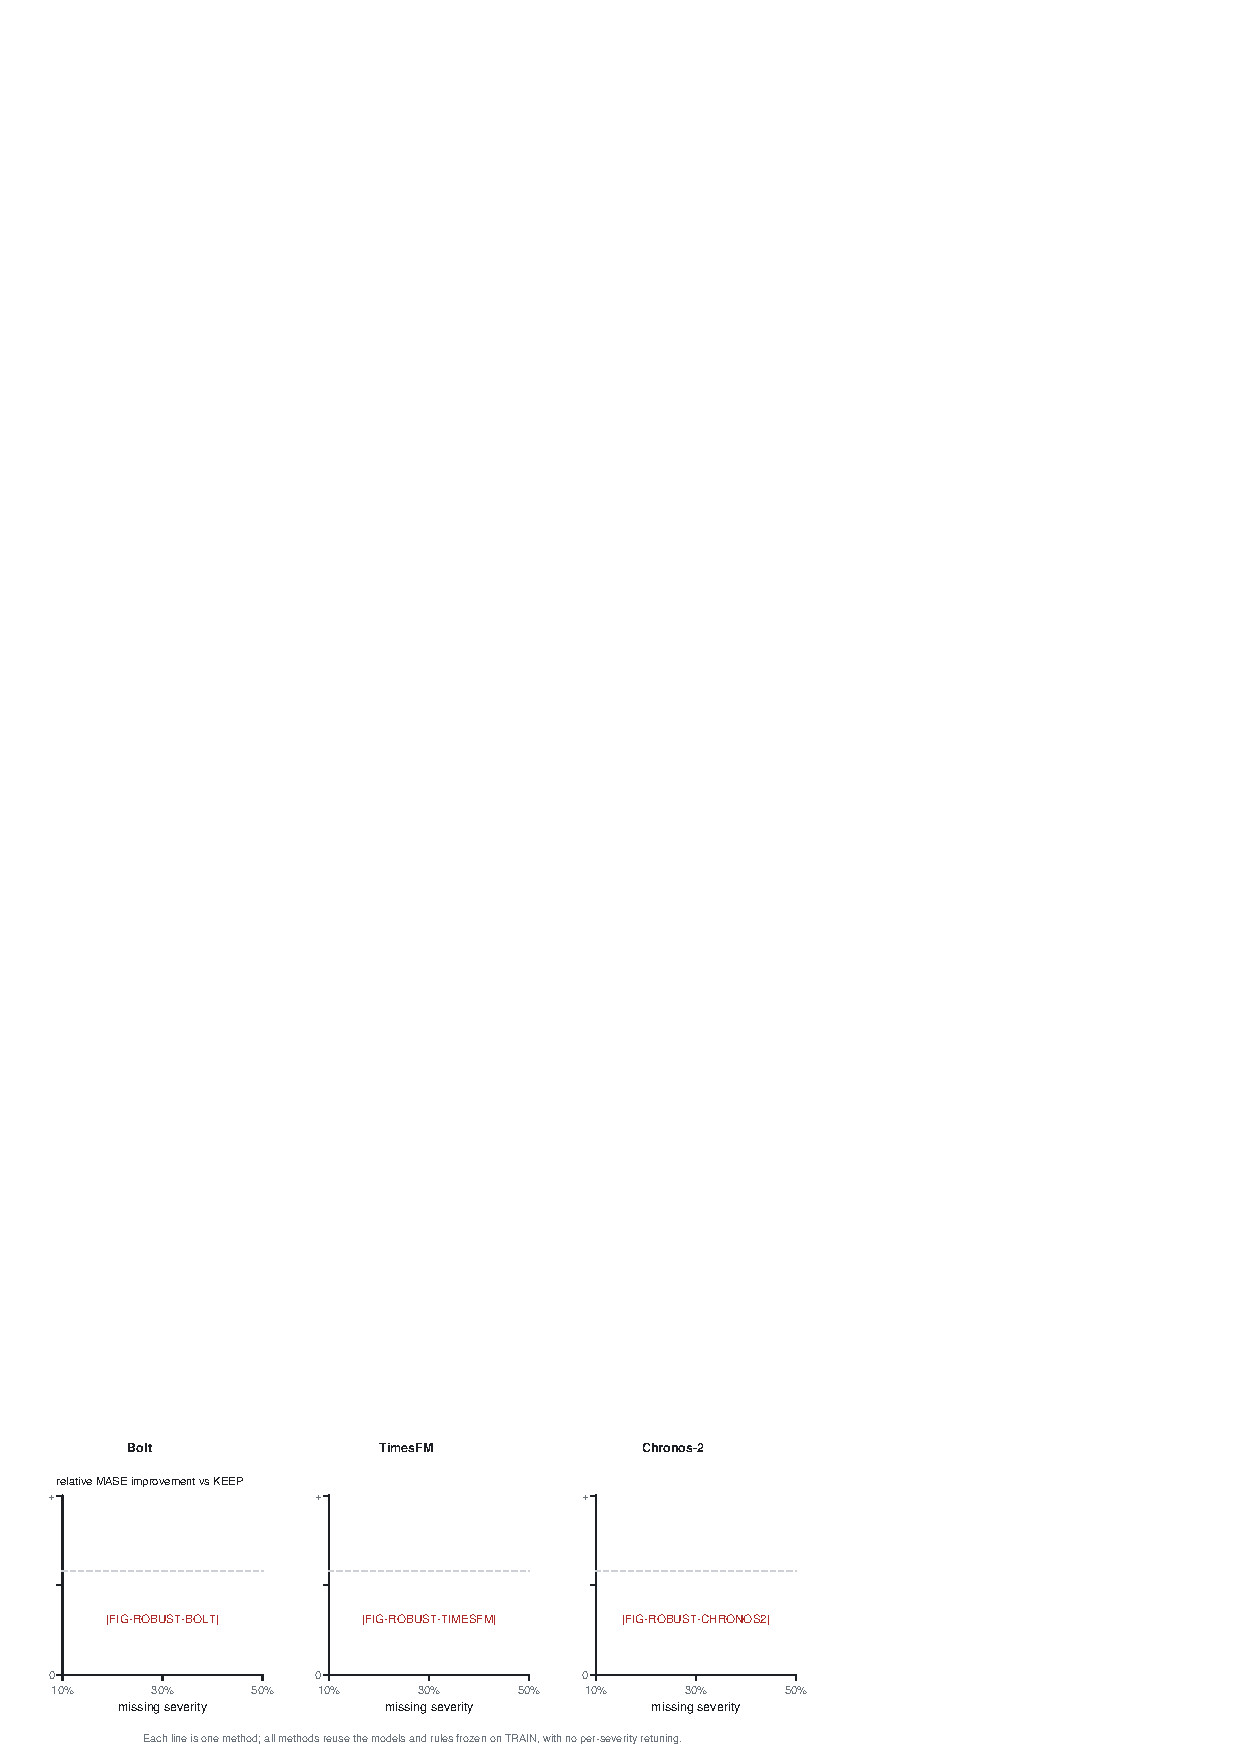
\includegraphics[width=0.86\textwidth]{figure/fig5_robustness_missingness.pdf}
  \caption{Relative MASE improvement over \textsc{Native Keep} as missingness severity
  increases, one line per method, one panel per frozen backbone. All methods reuse the
  models and rules frozen on TRAIN, with no per-severity retuning.}
  \label{fig:robust}
\end{figure}



\section{Reconstruction and Utility Diagnostics}
\label{app:diagnostics}
\subsubsection{Reconstruction versus Forecasting Utility}
\label{app:recutils}
This subsection supports \S\ref{sec:exp-exists}. Reconstruction error is defined only where a
method emits an explicit estimate of the hidden positions, which the four catalog interventions
and the published reconstruction baseline all do. Running the comparison on the catalog keeps both criteria on one protocol and
one set of episodes: the same window, the same mask, the same frozen backbone, and the same
realised future. \textsc{Keep} does not enter, because it estimates nothing, and \introact{}
does not enter, because it returns a forecast from an executed input rather than a
reconstruction.

Reconstruction error is measured on the artificially hidden positions of the target channel,
which are known because the mask is synthetic. Realised utility is the change in forecasting
loss the same action produced on the same episode. Both rankings are formed inside an episode
and then compared, because episodes differ in scale and in difficulty and pooling them would
let a few large-scale sources decide the answer. Table~\ref{tab:app-recutils} gives the
per-action averages and the two rank statistics.

\begin{table}[h]
  \caption{Reconstruction quality against realised forecasting utility, over the four catalog
  interventions and SAITS on the held-out evaluation episodes. Reconstruction error is measured on the
  hidden positions and realised utility against \textsc{Keep} on the same backbone. Winner
  agreement is the share of episodes on which the most accurate reconstruction is also the most
  useful intervention, and the discordant rate is the share of ordered pairs whose two rankings
  disagree.}
  \label{tab:app-recutils}
  \centering
  \small
  \setlength{\tabcolsep}{4pt}
\resizebox{\textwidth}{!}{\begin{tabular}{lcccc}
    \toprule
    Intervention & Rec.\ MSE $\downarrow$ & Rec.\ MAE $\downarrow$
                 & Mean realised utility $\uparrow$ & Episodes \\
    \midrule
    \textsc{Ffill}         & 77.47  & 4.08  & -0.139  & 760 \\
    \textsc{Single TS-ICL} & 29.61 & 2.03 & +0.013 & 760 \\
    \textsc{Multi TS-ICL}  & 29.52  & 1.85  & +0.033  & 760 \\
    \textsc{Context Ridge} & 30.19  & 1.47  & +0.052  & 570 \\
    SAITS                  & 77.60  & 3.35  & 0.000  & 760 \\
    \midrule
    \multicolumn{5}{l}{\footnotesize Winner agreement 21.1\%, discordant rate
    43.9\%, mean within-episode Spearman $\rho$ 0.13} \\
    \bottomrule
  \end{tabular}}
\end{table}

The averages in the table make the same point as the rank statistics. The intervention with the
lowest mean reconstruction error is not the one with the highest mean realised utility, so the
disagreement is not a property of a few unusual episodes. A deployment that picked its repair
by reconstruction accuracy would therefore be optimising a criterion that is close to
uninformative about the quantity it cares about.

\subsubsection{Where an Action's Utility Comes From}
\label{app:utility-by-severity}
Table~\ref{tab:app-utility-severity} reports the mean realised utility of each catalog action
on the replay bank, once over the whole bank and once within each registered severity. It
selects nothing and is computed after the configuration was frozen. Two things in it matter for
reading the main tables.

The first is that how much a repair is worth depends on the backbone and on how much of the
context is missing, and the two dependencies are not the same shape. On TimesFM every
non-trivial repair grows more valuable as the context empties, so a rule tuned at one severity
is looking at a moving target. On Chronos-2 the same repairs sit at roughly the same value
across severities. That is the premise of \S\ref{sec:exp-exists} restated as a table, and it is
why the decision cannot be a single policy learned once.

The second is a data-quality fact that has to travel with the numbers. On Bolt the mean utility
of \textsc{Context Ridge} over the whole bank is -0.372, while within the $10\%$
episodes alone it is +0.042. The gap is one replay episode on which the ridge
extrapolation diverged, and a single such record moves a mean over a few hundred. It was not
winsorised, because silently transforming a recorded execution is exactly what the protocol
forbids, and it is one reason the neighbourhood size matters: a local estimate over eight
neighbours is exposed to an outlier that an estimate over sixty-four dilutes.

\begin{table}[h]
  \caption{Mean realised utility of each action on the replay bank, overall and within each
  registered severity. Positive means the action lowered the forecasting loss relative to
  leaving the input unchanged. Utility is measured per episode, so it is not on the same
  aggregation as the source-macro MASE of the main tables and the two are not directly
  comparable in magnitude.}
  \label{tab:app-utility-severity}
  \centering
  \small
  \setlength{\tabcolsep}{4pt}
\resizebox{\textwidth}{!}{\begin{tabular}{llcccc}
    \toprule
    Backbone & Action & All severities & $10\%$ & $30\%$ & $50\%$ \\
    \midrule
    \multirow{4}{*}{Bolt}
      & \textsc{Ffill}         & -0.170  & -0.113  & -0.176  & -0.221 \\
      & \textsc{Single TS-ICL} & +0.026 & +0.017 & -0.003 & +0.063 \\
      & \textsc{Multi TS-ICL}  & +0.042  & +0.033  & +0.042  & +0.052 \\
      & \textsc{Context Ridge} & -0.372  & +0.042  & -1.370  & +0.154 \\
    \midrule
    \multirow{4}{*}{TimesFM}
      & \textsc{Ffill}         & -0.018  & -0.010  & -0.022  & -0.022 \\
      & \textsc{Single TS-ICL} & +0.205 & +0.112 & +0.198 & +0.300 \\
      & \textsc{Multi TS-ICL}  & +0.210  & +0.138  & +0.217  & +0.274 \\
      & \textsc{Context Ridge} & +0.287  & +0.180  & +0.290  & +0.389 \\
    \midrule
    \multirow{4}{*}{Chronos-2}
      & \textsc{Ffill}         & -0.184  & -0.086  & -0.202  & -0.262 \\
      & \textsc{Single TS-ICL} & +0.023 & +0.032 & +0.025 & +0.013 \\
      & \textsc{Multi TS-ICL}  & +0.044  & +0.053  & +0.062  & +0.018 \\
      & \textsc{Context Ridge} & +0.102  & +0.088  & +0.113  & +0.105 \\
    \bottomrule
  \end{tabular}}
\end{table}

\subsubsection{Governance Diagnostics}
\label{app:governance-fig}
Figure~\ref{fig:governance} visualises the diagnostics tabulated in
Table~\ref{tab:harm}. Panel~(b) is a sign-agreement check rather than a calibration
curve: the ranking score is used only to order actions, and we do not claim that its magnitude
is a calibrated probability.

\begin{figure}[h]
  \centering
  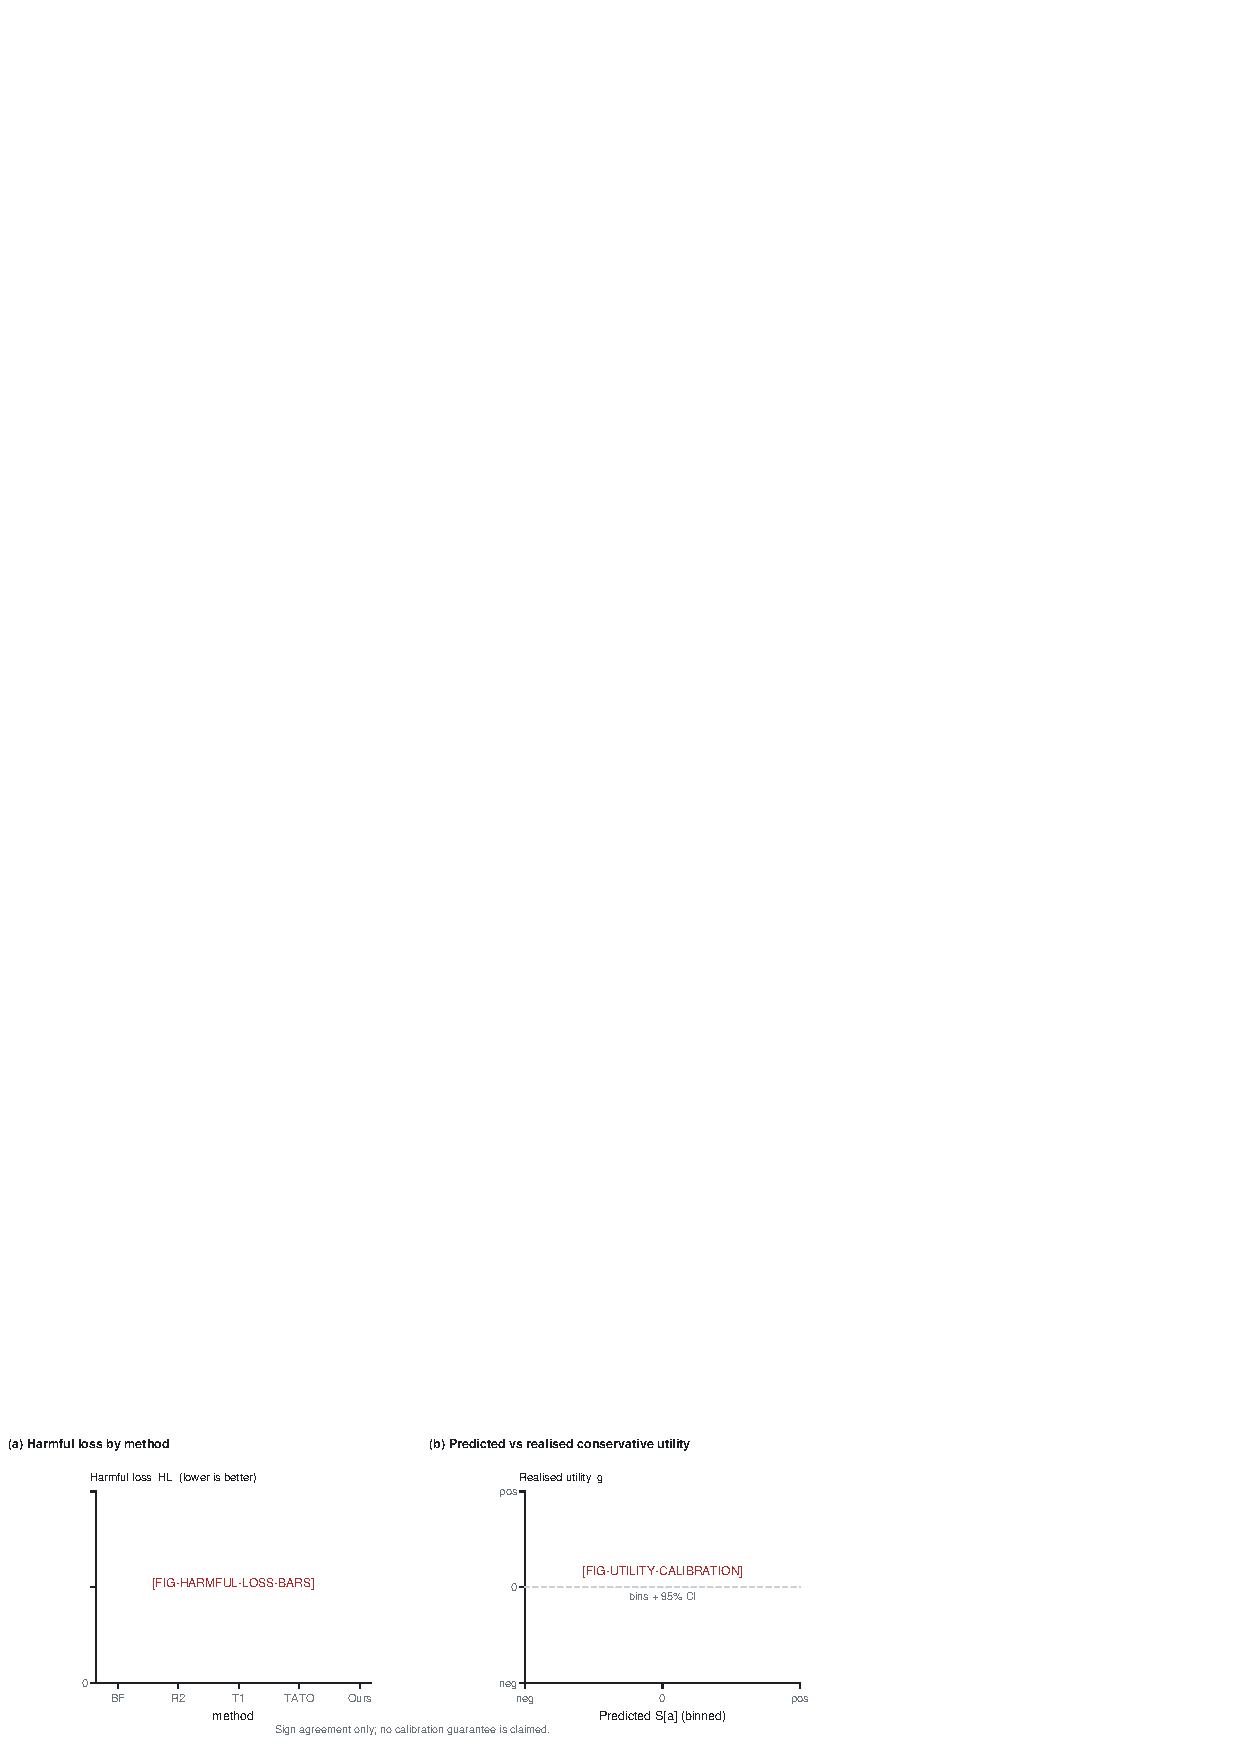
\includegraphics[width=0.84\textwidth]{figure/fig4_governance_diagnostics.pdf}
  \caption{\textbf{(a)}~Harmful loss by method. \textbf{(b)}~Realised utility against the
  binned ranking score with 95\% intervals. Panel~(b) is a sign agreement check, not a
  calibration claim.}
  \label{fig:governance}
\end{figure}



\section{Ablations and Stability}
\label{app:ablations-full}
\subsection{Ablation Details}
\label{app:ablation-details}
This section supports \S\ref{sec:exp-ablation}. Every variant reads the same catalog
prediction cache, so the rows differ only in how the stored utilities are summarised and
thresholded. Table~\ref{tab:app-ablation} reports the full outcome vector behind the compact
Table~\ref{tab:ablation}. The variant definitions follow \S\ref{sec:exp-ablation} exactly.

\begin{table}[h]
  \caption{Ablation, full outcome vector in the two scaled metrics. Raw errors are not
  averaged across sources anywhere in this paper, so they are not shown here either. Calls
  counts forecasting-backbone calls per request and harmful loss is relative to
  \textsc{Keep}.}
  \label{tab:app-ablation}
  \centering
  \small
  \setlength{\tabcolsep}{4pt}
\resizebox{\textwidth}{!}{\begin{tabular}{lcccccc}
    \toprule
    Variant & MASE $\downarrow$ & RMSSE $\downarrow$ & Intervention rate & Conditional HIR $\downarrow$ & Harmful loss $\downarrow$ & Calls $\downarrow$ \\
    \midrule
    Full \introact{}            & 1.447 & 1.239 & 82.6\% & 44.2\% & 0.0451 & 1.83 \\
    A1 Global utility & 1.462 & 1.246 & 100.0\% & 43.9\% & 0.0642 & 2.00 \\
    A2 w/o intervention state & 1.446 & 1.239 & 82.4\% & 43.8\% & 0.0460 & 1.82 \\
    A3 w/o reference-forecast state & 1.426 & 1.224 & 84.8\% & 42.6\% & 0.0426 & 1.85 \\
    A4 Always act & 1.439 & 1.233 & 100.0\% & 44.6\% & 0.0519 & 2.00 \\
    A5 Parametric utility predictor & 1.462 & 1.247 & 87.2\% & 44.0\% & 0.0574 & 1.87 \\
    \midrule
    \bottomrule
  \end{tabular}}
\end{table}

\subsection{Mask-Realisation Stability}
\label{app:seeds}
The main experiment uses one deterministic mask per parent. This appendix repeats the
comparison under two further deterministic mask realisations of the same parents, so that a
reader can see whether a conclusion depends on one particular realisation of the deletion
pattern. The three realisations are fixed before the run and are never treated as three
independent samples of parents: the statistical unit stays the parent, and the three
realisations are read as a stability check on the same parent set. Significance testing is
never performed across them.

The subset is fixed before the run: all eight sources, patterns P1 to P4, $10\%$ severity,
$H=96$, on Bolt and Chronos-2, and the comparison is restricted to \textsc{Keep}, R2-CART,
and \introact{}. Reporting the spread over three realisations is a stability diagnostic and
is not an additional estimate of variance.

\begin{table}[h]
  \caption{Mask-realisation stability. Each row is one deterministic mask realisation on the
  pre-registered subset. The spread across realisations is a stability diagnostic and is not
  an additional sample of parents.}
  \label{tab:app-seeds}
  \centering
  \small
  \setlength{\tabcolsep}{4pt}
\resizebox{\textwidth}{!}{\begin{tabular}{llccc}
    \toprule
    Backbone & Mask realisation & MASE $\downarrow$ & $\Delta$ vs \textsc{Keep} $\uparrow$ & Intervention rate \\
    \midrule
    Bolt      & primary seed        & 1.371 & -0.096 & 75.5\% \\
    Bolt      & second realisation  & 1.369 & -0.092 & 75.5\% \\
    Bolt      & third realisation   & 1.367 & -0.096 & 76.7\% \\
    \midrule
    Chronos-2 & primary seed        & 1.442 & -0.137 & 74.1\% \\
    Chronos-2 & second realisation  & 1.474 & -0.102 & 75.4\% \\
    Chronos-2 & third realisation   & 1.428 & -0.174 & 74.2\% \\
    \midrule
    \multicolumn{2}{l}{Spread over the three realisations (Bolt)}      & 0.003 & --- & 1.2\% \\
    \multicolumn{2}{l}{Spread over the three realisations (Chronos-2)} & 0.046  & --- & 1.3\% \\
    \bottomrule
  \end{tabular}}
\end{table}

\section{Cost, Failures, and Memory}
\label{app:cost-full}
\subsection{Runtime and Failure Audit}
\label{app:calls}
Table~\ref{tab:app-efficiency} gives the full cost breakdown behind the summary in
\S\ref{sec:exp-ablation}. Offline cost and online cost are kept in separate columns because
they are not directly comparable: the offline replay bank is built once per backbone revision,
per source, and per horizon, whereas the online columns are per request. Within each column a
lower value is better, and the two columns are read separately rather than combined into a
single score. Latency percentiles are measured per request and exclude cold start, which is
reported on its own line. Candidate materialisation is a separate line because it is paid
before the decision is made and is not a forecasting-backbone call.

\begin{table}[t]
  \caption{Deployment cost for the methods that carry a claim, offline and online kept
  separate. Latency percentiles are per request and exclude cold start, reported on its own
  line. Backbone calls counts forecasting-backbone calls per request and excludes candidate
  materialisation, which is reported in its own column.}
  \label{tab:app-efficiency}
  \centering
  \small
  \setlength{\tabcolsep}{4pt}
\resizebox{\textwidth}{!}{\begin{tabular}{lcccccc}
    \toprule
    Method & Offline train/search & Candidate constr. & Backbone calls/req.\ & Mean lat.\ $\downarrow$ & P95 $\downarrow$ & Max $\downarrow$ \\
    \midrule
    SAITS                 & 8 imputers, 3 min total     & 1 per request     & 1.00     & 52 ms     & 57 ms     & 469 ms \\
    TATO               & 3,072 calls, once per backbone   & 1 per request   & 1.00   & 52 ms   & 57 ms   & 469 ms \\
    \rowcolor{bestgray}\introact{} & 8,471 calls, once per backbone & 4 per request & 1.83 & 96 ms & 116 ms & 940 ms \\
    \midrule
    \multicolumn{7}{l}{\footnotesize Cold start: 3.4 s to load a backbone, paid once per process \quad
    Failure/timeout share: 0.00\%} \\
    \bottomrule
  \end{tabular}}
\end{table}

Table~\ref{tab:app-calls} separates offline from online cost and separates successes from
failures. Failures and timeouts are never counted as successes and are never dropped from the
denominator. A request that fails to produce a forecast is reported as a failure rather than
as a zero-cost success. A request costs one forecasting-backbone call for the reference action
and, when an intervention is executed, one further call for the selected action, so the online
count is between one and two backbone calls. When the decision returns \textsc{Keep} the input
is left untouched and the reference call is the returned forecast. Candidate materialisation
and scoring are booked on their own line because they are paid before the decision and do not
touch the backbone.

\begin{table}[h]
  \caption{Backbone call accounting. Latency is reported per request and excludes cold start,
  which is reported on its own line. The offline replay-bank build and the one-off selector fit
  are amortised and reported separately. Candidate materialisation and scoring are booked on
  their own line and are not forecasting-backbone calls.}
  \label{tab:app-calls}
  \centering
  \small
  \setlength{\tabcolsep}{4pt}
\resizebox{\textwidth}{!}{\begin{tabular}{lccc}
    \toprule
    Outcome & Requests & Share & Backbone calls per request \\
    \midrule
    \textsc{Keep} returned (input untouched)   & 132    & 17.4\%    & 1 \\
    Intervention executed (input changed)      & 628     & 82.6\%     & 2 \\
    Failed before any forecast                 & 0    & 0.00\%    & 0 \\
    Timed out after the forecast               & 0 & 0.00\% & 0 \\
    \midrule
    Candidate materialisation and scoring (per request) & 3,040 & --- & 0 \\
    Offline replay-bank build (amortised)      & --- & --- & 8,471 calls, once per backbone \\
    Offline selector fit (amortised)           & --- & --- & no fit; the selector stores the bank and retrieves from it \\
    Cold start (first request of a process)    & 15 & --- & 3.4 s \\
    \bottomrule
  \end{tabular}}
\end{table}

\section{Reproducibility and Artefact Schema}
\label{app:repro-full}
\subsubsection{Reproducibility Details}
\label{app:reprodetails}
Each record in the result files contains: source, parent, origin, horizon, pattern,
severity, mask hash, backbone, backbone revision, method, action, input hash, prediction
hash, forecast, target reference id, MASE, MSE, MAE, RMSE, reconstruction MSE where
applicable, runtime components, failure, fallback, code SHA, and the resolved configuration.
Results are written to the logical result groups listed in Table~\ref{tab:app-groups}, each in
CSV, JSON, and Markdown form, with raw predictions retained alongside the aggregates. The
group names describe the stage that produced them and do not encode a version number, so that
a later revision of the protocol cannot be confused with the present one.

\begin{table}[h]
  \caption{Result groups written by the pipeline. Every number in the main text and in the
  appendices is generated from one of these groups and nothing is transcribed by hand.}
  \label{tab:app-groups}
  \centering
  \small
  \setlength{\tabcolsep}{4pt}
\resizebox{\textwidth}{!}{\begin{tabular}{lll}
    \toprule
    Result group & Contents & Consumed by \\
    \midrule
    \texttt{protocol}       & frozen protocol, source manifests, split boundaries, TEST manifest & Appendix~\ref{app:splits} \\
    \texttt{replay\_bank}   & replay records $(z_{i,a}, a, g_{i,a})$ with input and prediction hashes & \S\ref{sec:method-replay} \\
    \texttt{baselines}      & baseline training runs, resolved hyperparameters, checkpoints & \S\ref{sec:exp-main} \\
    \texttt{train\_eval}    & TRAIN-eval acceptance check before freezing & Appendix~\ref{app:splits} \\
    \texttt{main\_results}  & main matrix rows, all methods, all cells & Tables~\ref{tab:main}, \ref{tab:app-src-bolt-96}--\ref{tab:app-src-ch2-192} \\
    \texttt{ablations}      & the five ablation variants and the catalog oracle diagnostic & Table~\ref{tab:ablation}, \ref{tab:app-ablation} \\
    \texttt{robustness}     & severity, pattern, and mask-realisation sweeps & Tables~\ref{tab:robust}, \ref{tab:app-sev10}--\ref{tab:app-sev50}, \ref{tab:app-seeds} \\
    \texttt{diagnostics}    & reconstruction and utility diagnostics, rank agreement & Appendix~\ref{app:diagnostics} \\
    \texttt{cost\_audit}    & call counts, latency, failures, timeouts, memory & Table~\ref{tab:app-efficiency}, Appendix~\ref{app:calls} \\
    \bottomrule
  \end{tabular}}
\end{table}

The protocol is frozen before the main experiment and identified by commit hash. Any change to
the action catalog, the missingness protocol, the mask derivation rule, the split boundaries,
the state feature list, or the failure policy invalidates the freeze and requires a new
configuration identifier. Calibration and TEST labels are not read during development, and no
result in this paper is selected on them.

\paragraph{Software and hardware.} Forecasts are produced with the released checkpoints of
Chronos-Bolt, TimesFM, and Chronos-2 at the revisions listed in Table~\ref{tab:app-repro}.
The surrounding code is Python 3.11.16 with NumPy 1.26.4, pandas
2.2.3, scikit-learn 1.5.2, and PyTorch 2.9.1+cu126. Runs are
executed on one NVIDIA RTX 4090 in bfloat16 for Chronos-Bolt, float32 for TimesFM and Chronos-2. The development-cycle numbers of
Appendix~\ref{app:development} were produced on a different machine and are not mixed with the
present results.

\begin{table}[h]
  \caption{Reproducibility anchors. Backbone revisions are the exact released checkpoints used
  for every forecast in this paper. Seeds are the deterministic seeds that fix the mask
  derivation, the replay-record ordering, and the selector fit.}
  \label{tab:app-repro}
  \centering
  \small
  \setlength{\tabcolsep}{4pt}
  \begin{tabular}{@{}l p{0.70\textwidth}@{}}
    \toprule
    Item & Value \\
    \midrule
    Chronos-Bolt revision   & amazon/chronos-bolt-base at 5d9f166d69f47aef3401367a7b842e78fe97b121 \\
    TimesFM revision        & TimesFM-2.5-200M, local snapshot pinned in the run ledger \\
    Chronos-2 revision      & amazon/chronos-2 at 29ec3766d36d6f73f0696f85560a422f50e8498c \\
    Python and libraries    & 3.11.16, NumPy 1.26.4, pandas 2.2.3, scikit-learn 1.5.2, PyTorch 2.9.1+cu126 \\
    Hardware and precision  & one NVIDIA RTX 4090, bfloat16 for Chronos-Bolt, float32 for TimesFM and Chronos-2 \\
    Mask derivation seed    & 20260917, a fixed literal rather than a clock reading \\
    Replay-record order seed & 101 \\
    Selector fit seed       & 101; the selector has no fitted parameters \\
    Protocol commit         & recorded with the run; see the released artefact ledger \\
    TEST manifest           & the TEST parents and origins listed in the evaluation records under results/v46/evaluation \\
    \bottomrule
  \end{tabular}
\end{table}

The TEST manifest is the authoritative record of which parents and origins were held out. It
is written once, before any result is computed, and every table in this paper is generated
against that manifest rather than against a split reconstructed after the fact.

\section*{Supplementary Exploratory Material}
\label{app:supplementary}
\subsection{Development Negative Results}
\label{app:development}
This section records what was tried earlier in this line of work and rejected. It is included
because the final formulation is easier to read against the alternatives it replaced, and
because omitting it would misrepresent how the method was reached. Nothing here is independent
confirmation of any method, and no number here is comparable with any table in the main text.

An earlier configuration tried to improve the action ranking by projecting estimated utility
vectors onto a convex feasible set before thresholding them. The projection reduced the squared
error of the estimated vector while failing to improve the final forecasting metric, and on one
backbone it degraded it. That outcome is the reason the present method ranks actions with a
local mean and a dispersion penalty and then applies a single threshold, rather than
calibrating a continuous score and reading a decision off it.

Two consequences of that cycle carry into the present paper. The strongest simple selector
available at the time, which is R2-CART in the present terminology, was competitive with the
more elaborate candidate, and on one backbone better than it, which is why R2-CART is carried
forward as a mandatory control in every main-text table. Reducing estimation error on a
continuous score was also not sufficient to improve discrete selection, which is why the
conservative gate is evaluated directly on harmful intervention rate and harmful loss rather
than on MASE alone.

The measurements behind that decision come from a different protocol, with a smaller
development split, fewer sources, and different budget accounting, so they are not reproduced
here as numbers. They are recorded in the released artefact ledger and must not be compared
numerically with any table in this paper.

\end{document}
